\documentclass[12,twoside]{mammeTFM}
\usepackage{amsthm,amsmath,amssymb,amsfonts,amscd}
\usepackage{enumerate}
\usepackage[all]{xy}
\usepackage{booktabs}
%\usepackage{fancyhdr}
\usepackage{algorithm}
\usepackage{algpseudocode}
\usepackage{tikz}

%%%%%Author packages if necessary
\usepackage{mathtools}


% Theorem Environments: add extra ones at the end if you need it.

\newtheorem*{theoremA}{Theorem A}
\newtheorem{theorem}{Theorem}[section]

\newtheorem{proposition}[theorem]{Proposition}
\newtheorem{lemma}[theorem]{Lemma}
\newtheorem{corollary}[theorem]{Corollary}
\newtheorem{conjecture}[theorem]{Conjecture}

\theoremstyle{definition}
\newtheorem{definition}[theorem]{Definition}
\newtheorem{example}[theorem]{Example}

\theoremstyle{remark}
\newtheorem{remark}[theorem]{Remark}
\newtheorem*{remarknonumber}{Remark}
\newtheorem{observation}[theorem]{Observation}

\usepackage{calc}
\usepackage{algorithmicx}
\newlength{\depthofsumsign}
\setlength{\depthofsumsign}{\depthof{$\sum$}}
\newlength{\totalheightofsumsign}
\newlength{\heightanddepthofargument}

\newcommand{\nsum}[1][1.4]{% only for \displaystyle
    \mathop{%
        \raisebox
            {-#1\depthofsumsign+1\depthofsumsign}
            {\scalebox
                {#1}
                {$\displaystyle\sum$}%
            }
    }
}


%%%%%%%%%%%%%%%%%%
% macros/abbreviations: Include here your own.
%%%%%%%%%%%%%%%%%%

\newcommand{\N}{\ensuremath{\mathbb{N}}}

% Body of document

\titol{Finding Partite Hypergraphs Efficiently}
\titolcurt{Finding Partite Hypergraphs Efficiently}
\authorStudent{Ferran Espuña Bertomeu}
\supervisors{Richard Lang}
\monthYear{June 2025}

%\msc[2010]{Primary 55M25, 57P10, Secondary 55P15, 57R19, 57N15.}

\paraulesclau{hypergraph, algorithm, graph, partite, extremal}
\agraiments{
Thanks to...}


\abstracteng{}

%%%%%%%%%
\begin{document}

\maketitle


\section{Introduction}\label{sec:introduction}

Graph theory provides fundamental tools for modeling relationships and networks across diverse fields.
A natural and powerful extension of graphs is the concept of \emph{hypergraphs},
where edges can connect more than two vertices.
Specifically, a $k$-uniform hypergraph, or $k$-graph,
consists of a set of vertices and a collection of edges, each being a $k$-element subset of the vertices.
For example, a $2$-graph is simply an undirected graph with no loops or parallel edges.
$k$-graphs arise naturally in areas ranging from combinatorics and computer science to data analysis and
computational biology.

A central branch is extremal (hyper)graph theory.
This field seeks to understand the maximum or minimum size of a combinatorial structure satisfying certain properties.
For instance, \emph{Turán-type problems} ask how many edges a $k$-graph can have, as a function of its number of vertices $n$,
without containing a specific subgraph $G$.
The maximum such number of edges is called the \emph{Turán number} of $G$ on $n$ vertices and is denoted by $\ex{n}{G}$.
A key result is Turán's Theorem~\cite{Turan1941},
which determines $\ex{n}{K_r}$ for all $n \geq r \geq 2$, where $K_r$ is the complete graph on $r$ vertices.
Furthermore, the Erdős--Stone--Simonovits Theorem~\cite{erdos1946structure}
asymptotically estimates $\ex{n}{G}$ for any fixed $2$-graph $G$ as $n \to \infty$,
and as a function of the chromatic number of $G$.

We do not yet understand how to extend these theorems to hypergraphs,
as the combinatorial structures become significantly more complex.
The asymptotic behavior of $\ex{n}{G}$ as $n \to \infty$
is characterized by the \emph{Turán density} of $G$, defined as
\[
    \pi(G) = \lim_{n \to \infty} \frac{\ex{n}{G}}{\binom{n}{k}}.
\]
Determining the exact value of $\pi(G)$ for $k$-graphs when $k > 2$
is a notoriously difficult open problem for many families,
including even small hypergraphs like the complete $3$-graph on $4$ vertices,
$K_4^{(3)}$~\cite{keevash2011hypergraph, razborov20103}.
This thesis focuses on the \emph{degenerate} case, where $\pi(G) = 0$.
A fundamental result states that this is the case if and only if $G$ is $k$-partite
(meaning its vertices can be partitioned into $k$ sets such that no edge has two vertices in the same set).
We are particularly interested in the problem of forbidding complete balanced $k$-partite $k$-graphs,
denoted $\compoverset{k}{t}$, which consist of $k$ disjoint sets of $t$ vertices each,
and all $t^k$ edges formed by selecting one vertex from each set.
The classical Kővari--Sós--Turán Theorem~\cite{Kovari1954, Hylten1958}
provides the following upper bound for $k=2$.
\[
    \ex{n}{K(s, t)} = \bigO{n^{2 - \frac{1}{\min\{s, t\}}}}.
\]
Erdős~\cite{Erods1964} found an analogous bound for complete balanced $k$-partite $k$-graphs for $k \ge 2$,
showing that
\begin{equation} \label{eq:erdos64-intro}
    \ex{n}{\compoverset{k}{t}} = \bigO{n^{k - \frac{1}{t^{(k-1)}}}}.
\end{equation}

Upper bounds for Turán numbers, like~\eqref{eq:erdos64-intro},
often involve counting or probabilistic arguments,
which are inherently non-constructive.
They guarantee the existence of the desired subgraph $\compoverset{k}{t}$
in dense enough hypergraphs but do not typically provide an efficient algorithm to \emph{find} such a subgraph.
If we focus on a fixed guest $k$-graph $G = (V, E)$ and let the number $n$ of vertices of the host $k$-graph $H$ grow,
this is not considered a problem,
as a brute-force search over all ordered sets of $|V|$ vertices in $H$ yields a polynomial-time algorithm
for finding a copy of $G$ in $H$.
However, the situation becomes more complex when we consider $G$ not to be fixed, but rather to grow with $n$.
We focus on the case where the edge density of $H$ is fixed (that is, $H$ has at least $\epsilon \binom{n}{k}$ edges),
and $G = \compoverset{k}{t}$ for some $t$ that can grow with $n$.
Careful analysis of the proof of Erdős' bound shows that this guarantees that $G$ is a subgraph of $H$ for some
\begin{equation} \label{eq:t-lower-intro}
    t = \delta(\epsilon) (\log n)^{\frac{1}{k-1}}.
\end{equation}
Running a brute-force search checking all $\binom{n}{kt}$ sets of $kt$
vertices in $H$ then does \textbf{not} yield a polynomial-time algorithm,
because $\binom{n}{kt}$ grows superpolynomially with $n$.

The main contribution of this thesis is bridging this gap by providing an efficient algorithmic solution.
We develop and analyze a deterministic, polynomial-time algorithm that,
given a $k$-graph $H$ with $n$ vertices and at least $dn^k$ edges (noting that $\binom{n}{k} \sim \frac{n^k}{k!}$
so $dn^k \sim \epsilon \binom{n}{k}$ for $\epsilon = k! d$)
finds a complete balanced $k$-partite subgraph $\compoverset{k}{t}$ within $H$, where
\[
    \left\lfloor \left(  \frac{\log \left(n/2^{(k-1)}\right)}{\log (3/d)} \right)^{\frac{1}{k-1}} \right\rfloor,
\]
matching the order of magnitude of~\eqref{eq:t-lower-intro}.
This result not only provides a constructive proof for the upper bounds of the type established by Erdős,
but in fact reaches the best possible value of $t$ up to a constant factor depending on $d$, as
can be shown by probabilistic arguments (see~\Cref{prop:probabilistic-lower-bound} and
the beginning of \Cref{sec:algorithm}, where the algorithm is introduced).
Our algorithm generalizes the approach used by Mubayi and Turán for the bipartite case ($k=2$)~\cite{MUBAYI2010174}.
It employs a recursive strategy that mirrors the inductive proof structure of Erdős' bound,
iteratively reducing the uniformity $k$ by constructing appropriate link graphs.

\textbf{Organization of the Thesis:}
\Cref{sec:preliminaries} formally introduces some families of hypergraphs
(including complete $k$-partite hypergraphs),
as well as basic operations like restrictions, links, and blow-ups.
We also use this section to introduce asymptotic notation, which is used throughout the thesis.
\Cref{sec:extremal} provides an overview of relevant theoretical results for Turán-type problems,
proving central theorems like the Turán Theorem (\Cref{thm:turan}), the Kővari--Sós--Turán Theorem (\Cref{thm:kst}),
Erdős' bound (\Cref{thm:erdos64}) and a more precise version of it (\Cref{thm:erdos64-constant-density}),
thus showing the existence a complete balanced $k$-partite subgraph of part sizes in the order of~\eqref{eq:t-lower-intro}
in $H$ when it has constant positive density.
\Cref{sec:algorithm} presents our main algorithm (\Cref{alg:kpartite}),
provides a rigorous proof of its correctness and analyzes its polynomial runtime complexity (\Cref{thm:kpartite}).
Finally, \Cref{sec:conclusions} summarizes the main results of this thesis, and discusses some open problems for future research.

% !TEX root = ../thesis.tex

\section{Hypergraph Turán Problems}\label{sec:preliminaries}
In this section we introduce some basic definitions and results that are used throughout this thesis.
We start with some preliminaries on hypergraphs, which are the main objects of study in this thesis.

\subsection{Hypergraphs}\label{subsec:hypergraphs}

\begin{definition}

    For an integer $k \geq 1$ a finite \emph{$k$-uniform hypergraph} (or \emph{$k$-graph}, for short)
    is a tuple $G = (V, E)$ where $V$ is a finite set
    and $E \subset \binom{V}{k}$.
    We call the elements of $V(G) = V$ its \emph{vertices}
    and those of $E(G) = E$ its \emph{edges}.
    The value $k$ is called the \emph{uniformity} of $G$.
\end{definition}

\begin{remark}
    In the definition above, if we let $k=1$, we get a set of $1$-sets of the vertex set $V$,
    which we can identify with a subset of $V$.
    If we let $k=2$, we recover the usual definition of an undirected graph with no loops.
\end{remark}

The following definition is a generalization of the notion of degree
of a vertex in a graph.

\begin{definition}
    Let $G = (V, E)$ be a $k$-graph and $v \in V$.
    The \emph{degree} $d_G(v)$ of $v$ in $G$
    is the number of edges containing $v$, that is
    \[
        d_G(v) = |\{e \in E \mid v \in e\}|.
    \]
\end{definition}

A useful operation is restricting a k-graph to a subset of its vertices.
This yields a new k-graph, called the \emph{subgraph induced by} the subset, which has the same uniformity.

\begin{definition}

    \label{def:restriction}
    Let $G = (V, E)$ be a $k$-graph and $T \subset V$.
    The \emph{restriction} of $G$ to $T$ is the $k$-graph
    \[
        G[T] = (T, E_T),
    \]
    where
    \[E_T = \{e \in E \mid e \subset T\}.\]
\end{definition}

The following operation also lets us obtain graphs of a
different uniformity from a subset of vertices of a $k$-graph.

\begin{definition} \label{def:link}
    Let $G = (V, E)$ be a $k$-graph.
    Let $1 \leq j \leq k - 1$ be an integer and let
    $T \subset V$ be a set of vertices satisfying $k - j \leq |T|$.
    The \emph{common $j$-link graph} of $T$ is the $j$-graph $\link{G}{T}{j} = (V \setminus T, E')$, where
    \[
        E' = \left\{Y \in \binom{V}{j}\middle\vert \, X \cup Y \in E \text{ for all } X \in \binom{T}{k-j}\right\}.
    \]
\end{definition}

\begin{figure}[htbp]
    \centering
    % TikZ code generated by Python script for Common Link Graph visualization
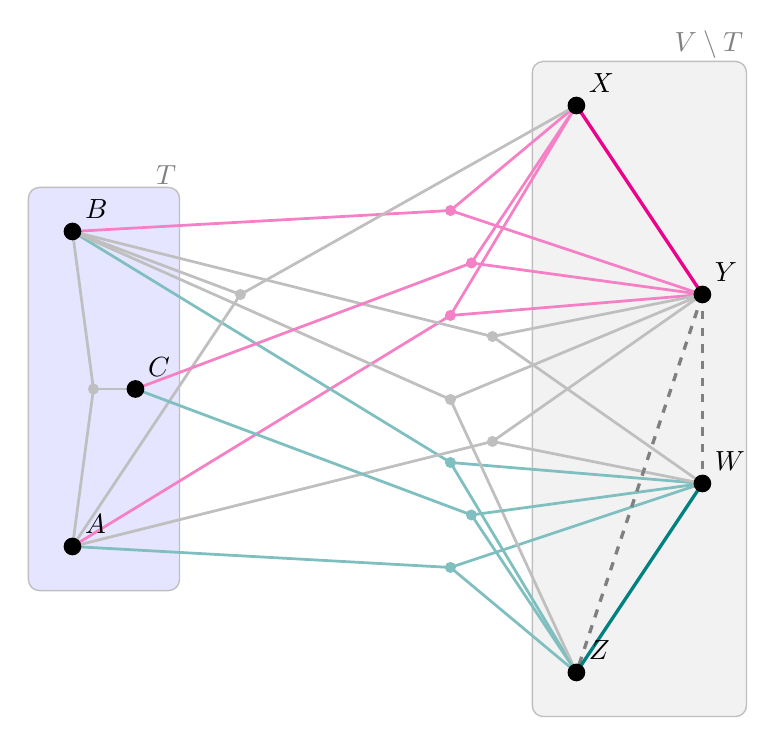
\begin{tikzpicture}[scale=0.8]
% Vertex coordinates
\coordinate (A) at (0.00, 2.00);
\coordinate (B) at (0.00, 7.00);
\coordinate (C) at (1.00, 4.50);
\coordinate (X) at (8.00, 9.00);
\coordinate (Y) at (10.00, 6.00);
\coordinate (Z) at (8.00, 0.00);
\coordinate (W) at (10.00, 3.00);
% Hyperedge root coordinates
\coordinate (R0) at (6.000, 5.667);
\coordinate (R2) at (6.000, 7.333);
\coordinate (R3) at (6.667, 5.333);
\coordinate (R4) at (6.000, 1.667);
\coordinate (R5) at (6.000, 3.333);
\coordinate (R6) at (2.667, 6.000);
\coordinate (R7) at (6.667, 3.667);
\coordinate (R8) at (6.000, 4.333);
\coordinate (R9) at (0.333, 4.500);
\coordinate (R10) at (6.333, 6.500);
\coordinate (R11) at (6.333, 2.500);
% Draw background boxes for T and V \ T
\draw[fill=blue!10, rounded corners, line width=0.5pt, draw=gray!50] (-0.70, 1.30) rectangle (1.70, 7.70);
\node at (1.70, 7.70) [anchor=south east, inner sep=1pt, text=gray] {$T$};
\draw[fill=gray!10, rounded corners, line width=0.5pt, draw=gray!50] (7.30, -0.70) rectangle (10.70, 9.70);
\node at (10.70, 9.70) [anchor=south east, inner sep=1pt, text=gray] {$V \setminus T$};
% Draw original hyperedges (styled by category)
\draw[line width=1.0pt, color=magenta!50!white, solid] (R0) -- (A);
\draw[line width=1.0pt, color=magenta!50!white, solid] (R0) -- (X);
\draw[line width=1.0pt, color=magenta!50!white, solid] (R0) -- (Y);
\fill[magenta!50!white] (R0) circle (2.5pt);
\draw[line width=1.0pt, color=magenta!50!white, solid] (R2) -- (B);
\draw[line width=1.0pt, color=magenta!50!white, solid] (R2) -- (X);
\draw[line width=1.0pt, color=magenta!50!white, solid] (R2) -- (Y);
\fill[magenta!50!white] (R2) circle (2.5pt);
\draw[line width=1.0pt, color=gray!50!white, solid] (R3) -- (B);
\draw[line width=1.0pt, color=gray!50!white, solid] (R3) -- (Y);
\draw[line width=1.0pt, color=gray!50!white, solid] (R3) -- (W);
\fill[gray!50!white] (R3) circle (2.5pt);
\draw[line width=1.0pt, color=teal!50!white, solid] (R4) -- (A);
\draw[line width=1.0pt, color=teal!50!white, solid] (R4) -- (Z);
\draw[line width=1.0pt, color=teal!50!white, solid] (R4) -- (W);
\fill[teal!50!white] (R4) circle (2.5pt);
\draw[line width=1.0pt, color=teal!50!white, solid] (R5) -- (B);
\draw[line width=1.0pt, color=teal!50!white, solid] (R5) -- (Z);
\draw[line width=1.0pt, color=teal!50!white, solid] (R5) -- (W);
\fill[teal!50!white] (R5) circle (2.5pt);
\draw[line width=1.0pt, color=gray!50!white, solid] (R6) -- (A);
\draw[line width=1.0pt, color=gray!50!white, solid] (R6) -- (B);
\draw[line width=1.0pt, color=gray!50!white, solid] (R6) -- (X);
\fill[gray!50!white] (R6) circle (2.5pt);
\draw[line width=1.0pt, color=gray!50!white, solid] (R7) -- (A);
\draw[line width=1.0pt, color=gray!50!white, solid] (R7) -- (Y);
\draw[line width=1.0pt, color=gray!50!white, solid] (R7) -- (W);
\fill[gray!50!white] (R7) circle (2.5pt);
\draw[line width=1.0pt, color=gray!50!white, solid] (R8) -- (B);
\draw[line width=1.0pt, color=gray!50!white, solid] (R8) -- (Y);
\draw[line width=1.0pt, color=gray!50!white, solid] (R8) -- (Z);
\fill[gray!50!white] (R8) circle (2.5pt);
\draw[line width=1.0pt, color=gray!50!white, solid] (R9) -- (A);
\draw[line width=1.0pt, color=gray!50!white, solid] (R9) -- (B);
\draw[line width=1.0pt, color=gray!50!white, solid] (R9) -- (C);
\fill[gray!50!white] (R9) circle (2.5pt);
\draw[line width=1.0pt, color=magenta!50!white, solid] (R10) -- (C);
\draw[line width=1.0pt, color=magenta!50!white, solid] (R10) -- (X);
\draw[line width=1.0pt, color=magenta!50!white, solid] (R10) -- (Y);
\fill[magenta!50!white] (R10) circle (2.5pt);
\draw[line width=1.0pt, color=teal!50!white, solid] (R11) -- (C);
\draw[line width=1.0pt, color=teal!50!white, solid] (R11) -- (Z);
\draw[line width=1.0pt, color=teal!50!white, solid] (R11) -- (W);
\fill[teal!50!white] (R11) circle (2.5pt);
% Draw 'almost' link edges (faintly, dotted)
\draw[color=gray, very thick, dashed] (Y) -- (Z);
\draw[color=gray, very thick, dashed] (Y) -- (W);
% Edges of the common 2-link graph of T (brightly colored)
\draw[very thick, color=magenta] (X) -- (Y);
\draw[very thick, color=teal] (Z) -- (W);
% Draw vertices (foreground layer)
\fill[black] (A) circle (4.0pt);
\node[above right=1pt, color=black] at (A) {$A$};
\fill[black] (B) circle (4.0pt);
\node[above right=1pt, color=black] at (B) {$B$};
\fill[black] (C) circle (4.0pt);
\node[above right=1pt, color=black] at (C) {$C$};
\fill[black] (X) circle (4.0pt);
\node[above right=1pt, color=black] at (X) {$X$};
\fill[black] (Y) circle (4.0pt);
\node[above right=1pt, color=black] at (Y) {$Y$};
\fill[black] (Z) circle (4.0pt);
\node[above right=1pt, color=black] at (Z) {$Z$};
\fill[black] (W) circle (4.0pt);
\node[above right=1pt, color=black] at (W) {$W$};
\end{tikzpicture}
    \caption{A $3$-graph $G$ and the common $2$-link graph $\link{G}{T}{2}$ of the set $T = \{A, B, C\}$.
        The link graph has vertex set $\{X, Y, Z, W\}$ and edge set
        $\{\{X, Y\}, \{W, Z\}\}$.
    }
    \label{fig:link}
\end{figure}

Figure~\ref{fig:link} exemplifies how to construct
a common $j$-link graph from a $k$-graph $G$ in the case $k=3$ and $j=2$.
Vertices are represented as black dots, and $3$-edges of $G$ are represented as colored or gray small dots,
connected by a line to the vertices they contain.
Colored dots correspond to $3$-edges with exactly
$k - j = 3 - 2 = 1$ vertices in $T$, which are the only ones that can contribute to the common $2$-link graph.
Edges in the common $2$-link graph are represented as solid lines connecting the corresponding vertices,
in the same color that the $3$-edges they come from.
Dashed lines correspond to edge pairs
in $V \setminus T$ that have some of the required $3$-edges in $G$, but not all of them.

\begin{remark}
    Definition~\ref{def:link} might appear confusing because $E'$ is defined
    as a set of subsets of $V$, while the link graph has vertex set $V \setminus T$.
    In fact, it is impossible for an element $Y \in E'$ to contain a vertex $v \in T$.
    To see this, suppose that $v \in Y$.
    We can pick a $(k-j)$-set $X \in \binom{T}{k-j}$ such that $v \in X$.
    Then $v \in X \cap Y$ so
    $| X \cup Y | < j + (k-j) = k$, contradicting the fact that $X \cup Y$ is an edge in $G$.
\end{remark}

Next, we introduce $k$-graph homomorphisms, embeddings and isomorphisms, which allow us
to relate $k$-graphs of the same uniformity to each other.

\begin{definition} \label{def:embedding}
    Let $G = (V, E)$ and $H = (W, F)$ be $k$-graphs and let $f: V \to W$ be a map
    between their vertex sets.
    If $A \subset E$ is a set of edges in $G$, we denote
    \[
        f(A) = \{f(e) \mid e \in A\} = \{\{f(v) \mid v \in e\} \mid e \in A\}.
    \]
    Then, $f$ is a \emph{homomorphism} from $G$ to $H$ if
    \begin{equation}
        \label{eq:homomorphism}
        f(E) \subset E(H[f(V)]).
    \end{equation}
    If such a homomorphism exists
    and is injective, we say that $f$ is an \emph{embedding} of $G$ on $H$
    and that $H$ \emph{contains} $G$ as a subgraph.
    We write $G \subset H$.
    If, furthermore,
    \begin{equation}
        \label{eq:induced_embedding}
        f(E) = E(H[f(V)]),
    \end{equation}
    we say that $f$is an \emph{induced} embedding
    and that $H$ contains $G$ as an \emph{induced} subgraph.
    We write $G \subset_{\text{ind}} H$.
    If, in addition, $f$ is a bijection, we say that $f$ is an \emph{isomorphism}
    and that $G$ is \emph{isomorphic} to $H$.
    We write $G \cong H$.
\end{definition}

\begin{remark}
    Condition~\eqref{eq:homomorphism} of definition~\ref{def:embedding}
    implies that $f$ is injective
    when restricted to each edge in $E$, because $G$ and $H$ have the same uniformity.
    However, it does not necessarily imply that $f$ is injective on all of $V$.
\end{remark}

\begin{remark} \label{rem:inverse_embedding}
    In Definition~\ref{def:embedding}, given that a map $f: V \to W$ is an embedding
    (and therefore injective),
    a different way to state that it is an induced embedding is to say that
    $f^{-1}: H[f(V)] \to G$ is also an embedding.
\end{remark}

For the notions that we have introduced to be useful,
we need to show some basic properties.

\begin{proposition}\label{prop:embedding_properties}
    Graph inclusion $(\subset)$ and induced graph inclusion $\left(\subset_{\text{ind}}\right)$
    are preorder relations on $k$-graphs.
    \begin{proof}
        We need to show that the relations are reflexive and transitive.
        Reflexivity is clear, as the identity map is an induced embedding of a $k$-graph in itself.
        Let $G, H,$ and $K$ be $k$-graphs with vertex sets $X, Y,$ and $Z$ respectively.
        If $G \subset H$ via $f: X \to Y$ and $H \subset K$ via $g: Y \to Z$,
        then $g \circ f: X \to Z$ is injective and satisfies that for each edge $e \in E(G)$,
        \[
            g \circ f(e) =
            \{g(f(x))\mid x \in e\} =
            \{g(y) \mid y \in f(e)\} \in E(K),
        \]
        because $f(e) \in E(H)$.
        Therefore, $G \subset K$ via $g \circ f$.
        If the embeddings are induced,
        and $e$ is an edge in
        $E(K[g \circ f(X)])$,
        then $e$ is also an edge in $E(K[g (Y)]) = g(E(H))$.
        Therefore, $e' = g^{-1}(e)$ is an edge in $H$.
        Furthermore, because $e = g(e') \subset g \circ f(X)$,
        we have that $e' \in E(H[f(X)]) = f(E(G))$,
        so $e \in g(f(E(G)))$.
    \end{proof}
\end{proposition}

\begin{proposition}\label{prop:isomorphism_equivalence}
    The relation of isomorphism $(\cong)$ is an equivalence relation on $k$-graphs.
    \begin{proof}
        The relation is reflexive via the identity map.
        If $f: G \to H$ is an isomorphism, then $f^{-1}: H \to G$ is also an isomorphism,
        so the relation is symmetric.
        Finally, if $f: G \to H$ and $g: H \to K$ are isomorphisms,
        then $g \circ f: G \to K$ is also an isomorphism, because it is bijective,
        and by Proposition~\ref{prop:embedding_properties},
        it is an embedding
        and $(g \circ f)^{-1} = f^{-1} \circ g^{-1}$ is also an embedding.
        By remark~\ref{rem:inverse_embedding}, we are done.
    \end{proof}
\end{proposition}

\begin{proposition} \label{prop:isomorphism_preserves_embedding}
    Let $G, G', H, H'$ be $k$-graphs such that $G \cong G'$ and $H \cong H'$.
    Then,
    \begin{enumerate}
        \item $G \subseteq H$ if and only if $G' \subseteq H'$. \label{item:embedding}
        \item $G \subseteq_{\text{ind}} H$ if and only if $G' \subseteq_{\text{ind}} H'$. \label{item:induced_embedding}
    \end{enumerate}
    \begin{proof} % TODO REVIEW
        Because the isomorphism relation is symmetric, we only need to show one direction of each implication.
        let $f: V(G) \to V(H)$ be an embedding of $G$ in $H$, and let
        $g: V(G) \to V(G')$ and $h: V(H) \to V(H')$ be isomorphisms between the respective graphs.
        We claim that the composition
        \[
            f' = h \circ f \circ g^{-1}: V(G') \to V(H')
        \]
        is an embedding of $G'$ in $H'$.
        Injectivity is given by the injectivity of $h, f$, and $g^{-1}$.
        By Proposition~\ref{prop:isomorphism_equivalence}, we have that $g^{-1}$ is an isomorphism of $G'$ in $G$,
        and in particular an embedding.
        Therefore, by Proposition~\ref{prop:embedding_properties},
        $f'$ is an embedding of $G'$ in $H'$, proving part~\eqref{item:embedding}.
        Suppose now that the embedding $f$ is induced.
        consider the maps
        \[
            (f')^{-1}: f'(V(G')) \to V(G')
        \]
        and
        \[
            \varphi = g \circ f^{-1} \circ h^{-1}: h \circ f(V(G)) \to V(G'),
        \]
        where we restrict the domain of $f^{-1}$ to $f(V(G))$.
        Because $g$ is a bijection, $V(G) = g^{-1}(V(G'))$ so the
        domain of $\varphi$ is $f'(V(G'))$.
        In fact, one can check that the two functions are identical.
        Because $f^{-1}$ is an embedding of $H[f(V(G))]$ in $G$,
        we can argue as in the first case that
        $(f')^{-1}$ is an embedding of $H'[f'(V(G'))]$ in $G'$,
        and therefore $f'$ is an induced embedding of $G'$ in $H'$.
        This concludes the proof of part~\eqref{item:induced_embedding}.
    \end{proof}
\end{proposition}

Propositions~\ref{prop:isomorphism_equivalence},~\ref{prop:embedding_properties},
and~\ref{prop:isomorphism_preserves_embedding}
establish that the properties of containing a $k$-graph $G$ as a (induced)
subgraph within a $k$-graph $H$ depend only on the isomorphism classes of $G$ and $H$.
Therefore, discussions of (induced) subgraph containment can be conducted up to isomorphism.

So far, we have not seen any concrete examples of $k$-graphs or their isomorphism classes.
We now introduce an important family of them.

\begin{definition} \label{def:complete}
    A $k$-graph $G = (V, E)$ is \emph{complete} if $E = \binom{V}{k}$.
    We denote $G = \completesuperindex{k}{V}$
\end{definition}

If $K$ and $K'$ are complete $k$-graphs with the same number of vertices $r$,
any bijection $f: V(K) \to V(K')$ is clearly an isomorphism between $K$ and $K'$.
This lets us talk, up to isomorphism, about \emph{the} complete $k$-graph on $r$ vertices $\completesuperindex{k}{r}$.
For example, in Figure~\ref{fig:complete_kgraph} we show the complete graph $\completesuperindex{3}{4}$.

\begin{figure}[htbp]
    \centering
    % TikZ code for K_4^(3) using predefined edge colors
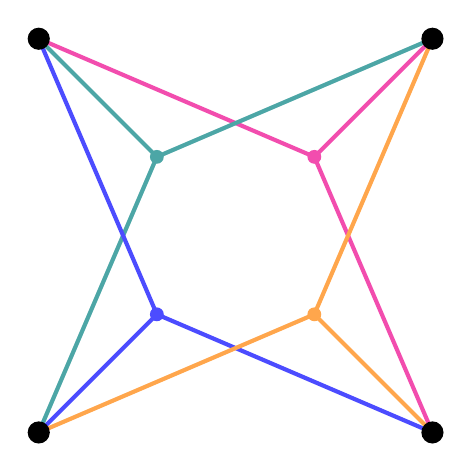
\begin{tikzpicture}[scale=1]
\coordinate (V1) at (0, 5);
\coordinate (V2) at (5, 5);
\coordinate (V3) at (5, 0);
\coordinate (V4) at (0, 0);
\coordinate (R0) at (3.500, 3.500);
\draw[line width=1.5pt, color=magenta!70!white] (R0) -- (V1);
\draw[line width=1.5pt, color=magenta!70!white] (R0) -- (V2);
\draw[line width=1.5pt, color=magenta!70!white] (R0) -- (V3);
\fill[color=magenta!70!white] (R0) circle (2.5pt);
\coordinate (R1) at (1.500, 3.500);
\draw[line width=1.5pt, color=teal!70!white] (R1) -- (V1);
\draw[line width=1.5pt, color=teal!70!white] (R1) -- (V2);
\draw[line width=1.5pt, color=teal!70!white] (R1) -- (V4);
\fill[color=teal!70!white] (R1) circle (2.5pt);
\coordinate (R2) at (1.500, 1.500);
\draw[line width=1.5pt, color=blue!70!white] (R2) -- (V1);
\draw[line width=1.5pt, color=blue!70!white] (R2) -- (V3);
\draw[line width=1.5pt, color=blue!70!white] (R2) -- (V4);
\fill[color=blue!70!white] (R2) circle (2.5pt);
\coordinate (R3) at (3.500, 1.500);
\draw[line width=1.5pt, color=orange!70!white] (R3) -- (V2);
\draw[line width=1.5pt, color=orange!70!white] (R3) -- (V3);
\draw[line width=1.5pt, color=orange!70!white] (R3) -- (V4);
\fill[color=orange!70!white] (R3) circle (2.5pt);
\fill[black] (V1) circle (4.0pt);
\fill[black] (V2) circle (4.0pt);
\fill[black] (V3) circle (4.0pt);
\fill[black] (V4) circle (4.0pt);
\end{tikzpicture}
    \caption{A complete $3$-graph on $4$ vertices.}
    \label{fig:complete_kgraph}
\end{figure}

\begin{remark}
    A $k$-graph $H = (V, E)$ contains $G = \completesuperindex{k}{r}$ as a subgraph if and only if,
    for some subset $T \subset V$ of size $r$, (namely, the image of an embedding of $G$)
    $H[T] \subset H$ is complete.
    Such an embedding is always induced, as it is given by the identity map on $T$.
\end{remark}

\subsection{Partite $k$-graphs}\label{subsec:partite}

We now introduce the notion of partite $k$-graphs.

\begin{definition} \label{def:partite}
    for an integer $p \geq k$, a $k$-graph $G = (V, E)$ is \emph{$p$-partite}
    (or $(p, 1)$-\emph{colorable})
    if there exists a partition $V = V_1 \cup \dots \cup V_p$
    such that every edge $e \in E$ intersects every part $V_i$ in at most one vertex.
    We may write $G = (V_1, \dots, V_p; E)$ and say that
    $G$ is a partite $k$-graph on $V_1, \dots, V_p$.
    If $p$ is the minimum integer such that $G$ is $p$-partite,
    we say that $p = \chi_{1}(G)$ is the \emph{partiteness} of $G$.
\end{definition}

The above definition is a special case of the family of chromatic numbers of hypergraphs $\chi_{\gamma}(G)$,
where we impose that an edge of the hypergraph can intersect each part in at most $\gamma$ vertices
(for example, see~\cite{krivelevich1998chromatic}).
If we set $\gamma = k - 1$, we recover the usual notion of chromatic number $\chi(G)$,
in which we impose that edges are not fully contained in any part.
In general, this is much weaker, but the two notions are the same when $k = 2$.

\begin{remark}
    These chromatic numbers are monotone non-decreasing with respect to the subgraph relation.
    Indeed, if $f: G \to H$ is an embedding of $k$-graphs,
    and $H$ is $(p, \gamma)$-partite with parts $V_1, \dots, V_p$,
    then $G$ is $(p, \gamma)$-partite with parts $f^{-1}(V_1), \dots, f^{-1}(V_p)$.
    This is because $f$ is injective, so it preserves the number of vertices in each part for every edge.
    This in turn means that $\chi_{\gamma}(G) \leq \chi_{\gamma}(H)$.
\end{remark}

If $G = (V_1, \dots, V_k; E)$ is a $k$-partite $k$-graph,
every edge intersects every part in exactly one vertex.
This means that we can identify the edges with a subset of $ V_1 \times \dots \times V_k$.
If it is clear from context, we may slightly abuse notation when talking about ordered and
unordered sets of vertices, as in the definition below.


\begin{definition} \label{def:complete_kpartite}
    A $k$-partite $k$-graph $G = (V_1, \dots, V_k; E)$ is \emph{complete}
    if $E = V_1 \times \dots \times V_k$.
    That is, if all $(v_1, \dots, v_k) \in V_1 \times \dots \times V_k$
    satisfy $\{v_1, \dots, v_k\} \in E$.
    We denote $G = \compdots{V_1}{V_k}$.
\end{definition}

In some cases, it is useful to generalize this notation to partite $k$-graphs
where the number of parts is different from $k$.

\begin{definition}
    Let $p \geq k \geq 1$.
    A $p$-partite $k$-graph $G = (V_1, \dots, V_p; E)$ is \emph{complete} if
    \[
        E = \bigcup_{\left\{i_1, \dots, i_k \right\} \in \binom{[p]}{k}} V_{i_1} \times \dots \times V_{i_k}.
    \]
    We denote $G = \compdotssuperindex{k}{V_1}{V_p}$.

\end{definition}

If $V_1, \dots, V_p$ and $W_1, \dots, W_p$ are disjoint sets
and $|V_i| = |W_i| = a_i$ for all $i$, then
\[
    \compdotssuperindex{k}{V_1}{V_p} \cong \compdotssuperindex{k}{W_1}{W_p}.
\]
An isomorphism is given by any bijection $f: V \to W$ (where $V=\cup_i V_i, W=\cup_i W_i$)
such that $f(V_i) = W_i$ for all $i$.
This allows us to talk, up to isomorphism, about \emph{the} complete $p$-partite $k$-graph
with part sizes $a_1, \dots, a_p$, which we denote by
\[
    \compdotssuperindex{k}{a_1}{a_p},
\]
or, in the $k$-partite case, by
\[
    K(a_1, \dots, a_k) = K^{(k)}(a_1, \dots, a_k).
\]

\begin{figure}[htbp]
    \centering
    % TikZ code for K^(3)(2, 2, 2) using predefined edge colors
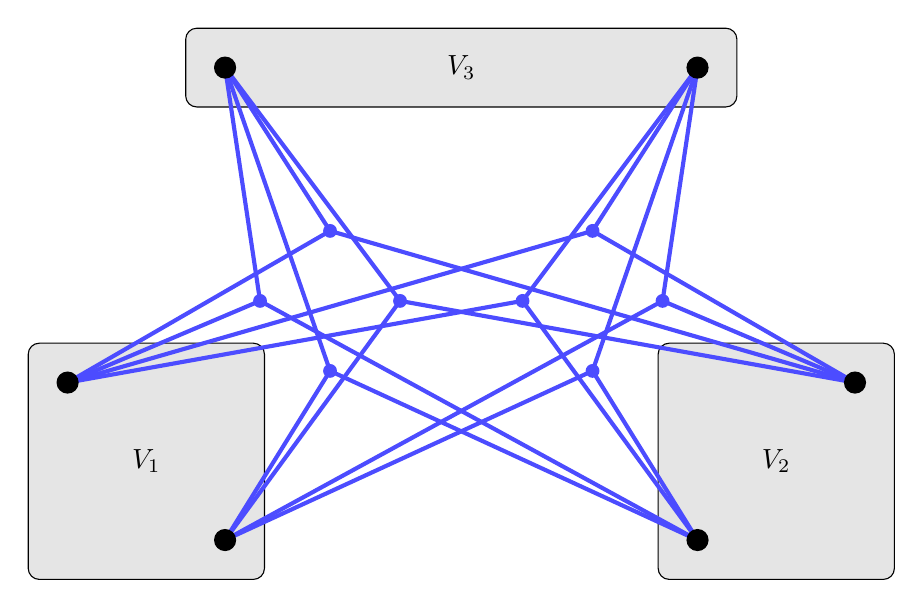
\begin{tikzpicture}[scale=1]
\draw[fill=gray!20, rounded corners] (-0.50, -0.50) rectangle (2.50, 2.50);
\node at (1.00, 1.00) [align=center] {$V_1$};
\draw[fill=gray!20, rounded corners] (7.50, -0.50) rectangle (10.50, 2.50);
\node at (9.00, 1.00) [align=center] {$V_2$};
\draw[fill=gray!20, rounded corners] (1.50, 5.50) rectangle (8.50, 6.50);
\node at (5.00, 6.00) [align=center] {$V_3$};
\coordinate (A1) at (2, 0);
\coordinate (A2) at (0, 2);
\coordinate (B1) at (8, 0);
\coordinate (B2) at (10, 2);
\coordinate (C1) at (2, 6);
\coordinate (C2) at (8, 6);
\coordinate (R0) at (3.333, 2.148);
\draw[line width=1.5pt, color=blue!70!white] (R0) -- (A1);
\draw[line width=1.5pt, color=blue!70!white] (R0) -- (B1);
\draw[line width=1.5pt, color=blue!70!white] (R0) -- (C1);
\fill[color=blue!70!white] (R0) circle (2.5pt);
\coordinate (R1) at (6.667, 2.148);
\draw[line width=1.5pt, color=blue!70!white] (R1) -- (A1);
\draw[line width=1.5pt, color=blue!70!white] (R1) -- (B1);
\draw[line width=1.5pt, color=blue!70!white] (R1) -- (C2);
\fill[color=blue!70!white] (R1) circle (2.5pt);
\coordinate (R2) at (4.222, 3.037);
\draw[line width=1.5pt, color=blue!70!white] (R2) -- (A1);
\draw[line width=1.5pt, color=blue!70!white] (R2) -- (B2);
\draw[line width=1.5pt, color=blue!70!white] (R2) -- (C1);
\fill[color=blue!70!white] (R2) circle (2.5pt);
\coordinate (R3) at (7.556, 3.037);
\draw[line width=1.5pt, color=blue!70!white] (R3) -- (A1);
\draw[line width=1.5pt, color=blue!70!white] (R3) -- (B2);
\draw[line width=1.5pt, color=blue!70!white] (R3) -- (C2);
\fill[color=blue!70!white] (R3) circle (2.5pt);
\coordinate (R4) at (2.444, 3.037);
\draw[line width=1.5pt, color=blue!70!white] (R4) -- (A2);
\draw[line width=1.5pt, color=blue!70!white] (R4) -- (B1);
\draw[line width=1.5pt, color=blue!70!white] (R4) -- (C1);
\fill[color=blue!70!white] (R4) circle (2.5pt);
\coordinate (R5) at (5.778, 3.037);
\draw[line width=1.5pt, color=blue!70!white] (R5) -- (A2);
\draw[line width=1.5pt, color=blue!70!white] (R5) -- (B1);
\draw[line width=1.5pt, color=blue!70!white] (R5) -- (C2);
\fill[color=blue!70!white] (R5) circle (2.5pt);
\coordinate (R6) at (3.333, 3.926);
\draw[line width=1.5pt, color=blue!70!white] (R6) -- (A2);
\draw[line width=1.5pt, color=blue!70!white] (R6) -- (B2);
\draw[line width=1.5pt, color=blue!70!white] (R6) -- (C1);
\fill[color=blue!70!white] (R6) circle (2.5pt);
\coordinate (R7) at (6.667, 3.926);
\draw[line width=1.5pt, color=blue!70!white] (R7) -- (A2);
\draw[line width=1.5pt, color=blue!70!white] (R7) -- (B2);
\draw[line width=1.5pt, color=blue!70!white] (R7) -- (C2);
\fill[color=blue!70!white] (R7) circle (2.5pt);
\fill[black] (A1) circle (4.0pt);
\fill[black] (A2) circle (4.0pt);
\fill[black] (B1) circle (4.0pt);
\fill[black] (B2) circle (4.0pt);
\fill[black] (C1) circle (4.0pt);
\fill[black] (C2) circle (4.0pt);
\end{tikzpicture}
    \caption{The complete 3-partite 3-graph $K(2, 2, 2)$, with parts $V_1, V_2, V_3$.}
    \label{fig:222}
\end{figure}

\begin{figure}[htbp]
    \centering
    % TikZ code for K^(2)(2, 2, 2) using predefined edge colors
\pgfdeclarelayer{background}
\pgfdeclarelayer{main}
\pgfsetlayers{background,main}
\begin{tikzpicture}[scale=0.8]
\begin{pgfonlayer}{background}
  \draw[fill=gray!20, rounded corners] (0.30, 0.30) rectangle (1.70, 3.70);
\end{pgfonlayer}
\node at (1.00, 2.00) [align=center] {$V_1$};
\begin{pgfonlayer}{background}
  \draw[fill=gray!20, rounded corners] (8.30, 0.30) rectangle (9.70, 3.70);
\end{pgfonlayer}
\node at (9.00, 2.00) [align=center] {$V_2$};
\begin{pgfonlayer}{background}
  \draw[fill=gray!20, rounded corners] (4.30, 5.30) rectangle (5.70, 8.70);
\end{pgfonlayer}
\node at (5.00, 7.00) [align=center] {$V_3$};
\coordinate (A1) at (1, 1);
\coordinate (A2) at (1, 3);
\coordinate (B1) at (9, 1);
\coordinate (B2) at (9, 3);
\coordinate (C1) at (5, 6);
\coordinate (C2) at (5, 8);
\draw[line width=1.5pt, color=magenta!60!white] (A1) -- (B1);
\draw[line width=1.5pt, color=magenta!60!white] (A1) -- (B2);
\draw[line width=1.5pt, color=magenta!60!white] (A2) -- (B1);
\draw[line width=1.5pt, color=magenta!60!white] (A2) -- (B2);
\draw[line width=1.5pt, color=teal!60!white] (A1) -- (C1);
\draw[line width=1.5pt, color=teal!60!white] (A1) -- (C2);
\draw[line width=1.5pt, color=teal!60!white] (A2) -- (C1);
\draw[line width=1.5pt, color=teal!60!white] (A2) -- (C2);
\draw[line width=1.5pt, color=orange!60!white] (B1) -- (C1);
\draw[line width=1.5pt, color=orange!60!white] (B1) -- (C2);
\draw[line width=1.5pt, color=orange!60!white] (B2) -- (C1);
\draw[line width=1.5pt, color=orange!60!white] (B2) -- (C2);
\begin{pgfonlayer}{main}
  \fill[black] (A1) circle (4.0pt);
  \fill[black] (A2) circle (4.0pt);
  \fill[black] (B1) circle (4.0pt);
  \fill[black] (B2) circle (4.0pt);
  \fill[black] (C1) circle (4.0pt);
  \fill[black] (C2) circle (4.0pt);
\end{pgfonlayer}
\end{tikzpicture}
    \caption{The complete 3-partite 2-graph $K^{(2)}(2, 2, 2)$, with parts $V_1, V_2, V_3$.}
    \label{fig:k2_222}
\end{figure}

Figure~\ref{fig:222} shows the complete $3$-partite $3$-graph
with $2$ vertices in each part, $K(2, 2, 2) = K^{(3)}(2, 2, 2)$.
In contrast, Figure~\ref{fig:k2_222} shows the complete $3$-partite $2$-graph
$K^{(3)}(2, 2, 2)$.

\subsection{Turán Problem for $k$-graphs}\label{subsec:turan}

Now we can state the \emph{forbidden subgraph problem} for $k$-graphs.
Informally, given a $k$-graph $G$, and an integer $n \geq |V(G)|$,
we want to find the smallest $M_0$ such that all $k$-graphs with $n$ vertices and $m > M_0$ edges
contain $G$ as a subgraph.

\begin{proposition} \label{prop:extremal}
    Let $G = (V, E)$ be a $k$-graph with nonempty edge set and $n \geq |V|$ be an integer.
    Then there exists an integer $M_0 = \ex{n}{G} \in \left[ 0, \binom{n}{k}\right)$ such that
    the condition
    \[
        \text{``All $k$-graphs with $n$ vertices and $m$ edges contain $G$ as a subgraph.''}
    \]
    is true for all $\binom{n}{k} \geq m > M_0$ and false for all $0 \leq m \leq M_0$.

    \begin{proof}
        Note that, if $M_0$ exists, clearly it is unique.
        Also, the condition is clearly false for $m = 0$ and
        true for $m = \binom{n}{k}$
        (the only graph $H$ with vertex set $W$, $|W|=n$ and $\binom{n}{k}$ edges
        is the one having all $k$-sets of vertices so any injective map $f: V \to W$
        is an embedding of $G$ in $H$).
        We only need to show that if the condition is true for $m$ then it is true for
        all $m' \geq m$.
        Suppose it is true for $m$ and let $m' \geq m$.
        Let $H = (W, F)$ be a $k$-graph with $n$ vertices and $m'$ edges.
        We can take $F' \subset F$ with $|F'| = m$.
        By hypothesis, the graph $H' = (W, F')$ contains $G$ as a subgraph,
        and the identity map in $W$ is an embedding of $H'$ in $H$.
        Then, $G \subset H' \subset H$ implies $G \subset H$ by transitivity of the embedding
        relation (Proposition~\ref{prop:embedding_properties}).

    \end{proof}

\end{proposition}

We call the integer $\ex{n}{G}$ the \emph{Turán number} of $G$ on $n$ vertices.
It is clearly invariant under isomorphism of $G$.
There are very few $k$-graphs $G$ for which an exact formula for $\ex{n}{G}$ is known.
Of these, the most famous family of examples are the complete $2$-graphs $\completesuperindex{2}{r}$,
for which extremal numbers were first studied by Turán~\cite{Turan1941} in 1941.
The result is the following.

\begin{theorem}[Turán Theorem]
    \label{thm:turan}
    Let $r > 2$ be an integer and let $n \geq r$.
    Let $a_1, \dots, a_{r-1}$ be integers such that $a_1 + \dots + a_{r-1} = n$
    and $\lfloor n / (r-1) \rfloor \leq a_i \leq \lceil n / (r-1) \rceil$ for all $i$.
    Then
    \begin{equation} \label{eq:turan}
        \ex{n}{\completesuperindex{2}{r}} = \sum_{\{x, y\} \in \binom{[r-1]}{2}} a_x \cdot a_y
    \end{equation}
    Furthermore, if $G$ is a $2$-graph with $\ex{n}{\completesuperindex{2}{r}}$ edges
    and $G$ does not contain $K_r^{(2)}$ as a subgraph, then
    \[
        G\cong \compdotssuperindex{2}{a_1}{a_{r-1}}.
    \]

\end{theorem}

To prove this theorem, we suppose that $G = (V, E)$ is a $2$-graph with $n$ vertices and
$\ex{n}{\completesuperindex{2}{r}}$edges, and use the following two lemmas.

\begin{lemma}\label{lem:same_degree}
    If $x, y \in V$ are different vertices and $\{x, y\} \notin E$, then $d_G(x) = d_G(y)$.
    \begin{proof}
        We argue by contradiction.
        Suppose, without loss of generality, that $d_G(x) > d_G(y)$.
        We argue that we can construct a $2$-graph $G'$ with $n$ vertices
        and more edges than $G$ that does not contain $K_r^{(2)}$ as a subgraph, against the definition of
        the Turán number.

        The new graph $G' = (E', V')$ is constructed from $G$ by removing from $V$ the vertex $y$
        (and all edges containing it)
        and adding a copy $x'$ of $x$, connected to the same vertices (that is, $\{x', v\} \in E'$
        if and only if $\{x, v\} \in E$).
        Clearly, $|V'| = |V|$ and $|E'| = E - d_G(y) + d_G(x) > |E|$.
        To see that $G'$ does not contain $K_r^{(2)}$ as a subgraph,
        suppose that $G'[T']$ is complete for some $T' \subset V'$ of size $r$.
        Because $\{x, x'\}$ is not an edge in $G'$, $T'$ cannot contain both $x$ and $x'$.
        Because the edges not containing $x'$ are the same as in $G$, which contains no $K_r^{(2)}$,
        we deduce that $T'$ contains $x'$ and therefore does not contain $x$.
        Now, let $T = (T' \setminus \{x'\}) \cup \{x\} \subset V$, also of size $r$.
        We argue that the graph $G[T] = G'[T]$ must be complete, reaching a contradiction.
        If it were not, then there would exist $v \in T, v \neq x$, such that $\{x, v\} \notin E$.
        This implies that $\{x', v\} \notin E'$, but $v \in T' \setminus \{x'\}$,
        against the completeness of $G'[T']$.
    \end{proof}
\end{lemma}

\begin{lemma} \label{lem:turan_complete_partite}
    $G$ is a complete $p$-partite graph for some $p \geq 2$.
    \begin{proof}
        Equivalently, we show that the relation defined by non-adjacency on $V$ (that is, $x \sim y$ when
        $\{x, y\} \notin E$) is an equivalence relation, so we can divide $V$ into equivalence classes
        by this relation, which means that $\{x, y\} \in E$ if and only if they are in different parts.

        The reflexivity and symmetry of the relation are clear.
        Suppose, by way of contradiction, that there exist $x, y, z \in V$ such that
        $x \sim z$ and $y \sim z$, but $x \nsim y$.
        We now construct a different graph $G'$ with the same number of vertices as $G$
        that also does not contain $K_r^{(2)}$ as a subgraph, reaching a contradiction.
        $G'$ is constructed from $G$ by removing the vertices
        $x$ and $y$ (and all the associated edges) and adding the two new vertices
        $z_1$ and $z_2$ and the edges $\{\{v, z_i\} | \{v, z\} \in E, i \in \{1, 2\}\}$.

        First, we show that $G'$ contains no embedding of $K_r^{(2)}$.
        We make a similar argument as in the proof of Lemma~\ref{lem:same_degree}.
        By way of contradiction, suppose that $G'[T']$ is complete for some $T' \subset V'$ of size $r$.
        Because $z$, $z_1$ and $z_2$ pairwise non-edges of $G'$, only one of them can be
        an image of a vertex in $K_r^{(2)}$.
        However, $G'[V \setminus \{x, y\}] \subset G$ has no embedding of $K_r^{(2)}$,
        so at least one of the vertices in $K_r^{(2)}$ must be mapped to $z_1$ or $z_2$.
        Without loss of generality, we can write $T' = \{x_1, x_2, x_3, \dots, x_{r-1}, z_1\}$,
        with $x_i \notin \{z_2, z\}$ for all $i$.
        However, $\{z_1, x_i\}$ is an edge in $G'$ if an only if $\{z, x_i\}$ is an edge in $G$,
        which means that $G'[\{x_1, x_2, x_3 \dots, x_{r-1}, z\}] = G[\{x_1, x_2, x_3 \dots, x_{r-1}, z\}]$ is complete,
        against our assumption.

        Now, we show that $G'$ has more edges than $G$.
        By Lemma~\ref{lem:same_degree}, $d_G(x) = d_G(z)$ and $d_G(y) = d_G(z)$,
        so the three vertices $x, y, z$ have the same degree $d$ in $G$.
        The edges containing $x$ and the edges containing $y$ intersect at exactly the edge $\{x, y\} \in E$.
        Therefore, by removing all of them from $G$ we are removing $2d - 1$ edges.
        Furthermore, for each edge containing $z$ we are adding two edges,
        and these sets of edges do not intersect because $z$ is not adjacent to $x$ or $y$ (so $\{z_1, z_2\} \notin E'$).
        We conclude that $G'$ has $|E'| = |E| - (2d - 1) + 2d = |E| + 1 > |E| $ edges, as we wanted to show.
    \end{proof}
\end{lemma}

Now we are ready to prove Theorem~\ref{thm:turan}.
\begin{proof}[Proof of Turán Theorem]
    We have shown in Lemma~\ref{lem:turan_complete_partite} that $G = (V_1, \dots V_p; E)$ is complete.
    In fact, we can set $p = r - 1$:
    If $p < r - 1$, we can always add empty parts to $G$; and if it has more than $r - 1$ nonempty parts
    (without loss of generality, $x_1 \in V_1, \dots, x_r \in V_r$), then $G[\{x_1, \dots, x_r\}]$ is complete,
    which is a contradiction.
    Furthermore, any complete $(r-1)$-partite $2$-graph is $\completesuperindex{2}{r}$-free,
    because $\completesuperindex{2}{r}$ is not $(r-1)$-partite.

    This means that we only need to show that the choice of the part sizes $a_1, \dots, a_{r-1}$ summing to $n$
    in the statement maximizes the expression~\eqref{eq:turan}.
    The imposition that $\lfloor n / (r-1) \rfloor \leq a_i \leq \lceil n / (r-1) \rceil$ for all $i$
    is equivalent to saying that the part sizes are as equal as possible, that is,
    $|a_i - a_j| \leq 1$ for all $i, j$.
    Suppose, by way of contradiction and without loss of generality, that $a_1 > a_2 + 1$.
    Let $a_1' = a_1 - 1$, $a_2' = a_2 + 1$ and $a_i' = a_i$ for all $i \geq 3$.
    Then,
    \begin{align*}
        \sum_{\{x, y\} \in \binom{[r-1]}{2}} a_x' \cdot a_y'
        =& \, (a_1 - 1)(a_2 + 1) + (a_1 - 1) \sum_{i \geq 3} a_i + (a_2 + 1) \sum_{i \geq 3} a_i + \sum_{3 \leq x < y} a_x a_y \\
        =& \sum_{\{x, y\} \in \binom{[r-1]}{2}} a_x \cdot a_y - a_2 + a_1 - 1
        > \sum_{\{x, y\} \in \binom{[r-1]}{2}} a_x \cdot a_y,
    \end{align*}
    in contradiction with the number of edges in $G$ being maximal.
\end{proof}

Because of the difficulty of finding exact extremal numbers for $k$-graphs,
we usually look for asymptotic approximations of them.
In particular, we are interested in how the expression
$\ex{n}{G}$ grows with $n$ for any fixed $k$-graph $G$.
This is known as the \emph{Turán problem} for the graph $G$.
For an example, we turn to the complete $2$-graph $\completesuperindex{2}{r}$,
for which we already have an exact formula.
In expression~\eqref{eq:turan}, we can see that
$a_i = n/(r-1) + \bigO{1}$ for all $i$.
Therefore,
\begin{equation} \label{eq:turan_asymptotic}
    \ex{n}{\completesuperindex{2}{r}} = \sum_{\{x, y\} \in \binom{[r-1]}{2}} a_x \cdot a_y
    = \binom{r-1}{2} \cdot \left( \frac{n}{r-1} + \mathcal{O}(1) \right)^2
    = \frac{(r-2)}{2(r-1)} n^2 + \mathcal{O}(n).
\end{equation}
Note that the maximum number of edges in a $2$-graph on $n$ vertices is
\[
    \binom{n}{2} = \frac{1}{2} n^2 + \mathcal{O}(n).
\]
The two quantities are comparable as they are both quadratic in $n$.
This lets us restate equation~\eqref{eq:turan_asymptotic} as
\begin{equation} \label{eq:turan_asymptotic_density}
    \ex{n}{\completesuperindex{2}{r}} =
    \frac{r-2}{r-1} \binom{n}{2} + \mathcal{O}(n) =
    \frac{r-2}{r-1} \binom{n}{2} + o\left(\binom{n}{2}\right),
\end{equation}
Which means that, asymptotically, the maximum \emph{edge density} of a $2$-graph on $n$ vertices
without $K_r^{(2)}$ as a subgraph is $(r-2)/(r-1) < 1$, so we must exclude a nontrivial fraction of edges
to avoid any particular complete $2$-graph.
The following general theorem greatly restricts the growth of Turán numbers
for all $k$-graphs.

\begin{theorem}
    Let $G = (V, E)$ be a $k$-graph.
    The limit
    \begin{equation} \label{eq:turan_density}
        \pi(G) = \lim_{n \to \infty} \frac{\ex{n}{G}}{\binom{n}{k}}
    \end{equation}
    exists and is between $0$ and $1$.
    We call it the \emph{Turán density} of $G$.
    \begin{proof}
        The sequence
        \[
            a_n = \frac{\ex{n}{G}}{\binom{n}{k}}
        \]
        Is bounded between $0$ and $1$ for all $n \geq |V(G)|$, by Proposition~\ref{prop:extremal}.
        Furthermore, it is less than $1$ for all $n \geq |V(G)| + 1$.
        To see this, consider a graph $H = (W, F)$ with $n$ vertices and $\binom{n}{k} - 1$ edges.
        Its edge density is less than $1$.
        Without loss of generality, we can suppose that $F = \binom{W}{k} \setminus \{\{x, y\}\}$.
        This means that $H[W \setminus \{x\}]$ is a complete $k$-graph on $n - 1$ vertices,
        which must contain $G$ as a subgraph.

        We show that the sequence $(a_n)$ is non-increasing, so it must converge to a value $0 \leq \pi(G) < 1$.
        Let $n \geq |V(G)|$.
        There exists a graph $H = (W, F)$ with $n+1$ vertices and $\ex{n+1}{G}$ edges that does not contain
        $G$ as a subgraph.
        For each vertex $w \in W$, the graph $H_w = H[W \setminus \{w\}]$ has $n$ vertices
        and does not contain $G$ as a subgraph.
        Therefore, it must contain at most $\ex{n}{G}$ edges.
        Consider the set
        \[
            \mathcal{P} = \left\{ (w, e) | w \in W, e \in E(H_w) \right\}.
        \]
        Counting on the first coordinate, we get
        \begin{equation} \label{eq:densityUpperBound}
            |\mathcal{P}| = \sum_{w \in W} |E(H_w)| \leq (n+1)\, \ex{n}{G}.
        \end{equation}
        On the other hand, for every edge $e \in F$, $e \in E(H_w)$
        for all $w \in W \setminus e$.
        Therefore, counting on the second coordinate, we get
        \begin{equation} \label{eq:densityLowerBound}
            |\mathcal{P}| = (n + 1 - k) |F| = (n + 1 - k)\, \ex{n+1}{G}.
        \end{equation}
        Combining equations~\eqref{eq:densityUpperBound} and~\eqref{eq:densityLowerBound},
        we get
        \[
            (n + 1 - k)\, \ex{n+1}{G} \leq (n + 1)\, \ex{n}{G}.
        \]
        Going back to the sequence $a_n$, we can write
        \[
            a_{n+1} = \frac{\ex{n+1}{G}}{\binom{n+1}{k}} \leq
            \frac{(n + 1)\, \ex{n}{G}}{(n + 1 - k) \binom{n+1}{k}} =
            \frac{\ex{n}{G}}{\binom{n}{k}} = a_n. \qedhere
        \]
    \end{proof}
\end{theorem}

We can now summarize expression~\eqref{eq:turan_asymptotic_density} as follows.
\begin{corollary} \label{cor:turan_density_kr}
    The Turán density of the complete $2$-graph $\completesuperindex{2}{r}$ is
    \[
        \pi\left(\completesuperindex{2}{r}\right) = \frac{r-2}{r-1} = 1 - \frac{1}{r-1}.
    \]
\end{corollary}

The first natural question that arises is for what graphs $G$ the Turán density $\pi(G)$ is positive
(in which case, we call the corresponding Turán problem \emph{non-degenerate}
and consider it solved if we can calculate $\pi(G)$).
The following gives a complete characterization.

\begin{proposition} \label{prop:degenerate}
    Let $G = (V, E)$ be a $k$-graph.
    Then $\pi(G) = 0$ if and only if $G$ is $k$-partite.
    \begin{proof}
        If $G$ is not $k$-partite, a construction similar to the one in the proof of Theorem~\ref{thm:turan}
        directly shows $\pi (G) > 0$.
        Indeed, for all $m$ the graph $\compoverset{k}{m}$ is $k$-partite so it cannot contain $G$ as a subgraph.
        Furthermore, its edge density is
        \[
             \frac{m^k}{\binom{km}{k}} \geq \frac{1}{k^k}.
        \]
        Because we can make $n = km = |V\left( \compoverset{k}{m} \right)|$ as large as we want,
        the limit~\eqref{eq:turan_density} bounded below by a positive constant.
        We defer the proof of the other direction to subsection~\ref{subsec:degenerate},
        where we study $k$-partite $k$-graph Turán problems
        in more depth (in particular, see Theorem~\ref{thm:erdos64}).
    \end{proof}
\end{proposition}

In fact, non-degenerate Turán problems for $2$-graphs are considered solved in this regard.
The following theorem gives the Turán density of all $2$-graphs.

\begin{theorem}[Erdős-Stone-Simonovits Theorem]
    \label{thm:erdos_stone_simonovits}
    Let $G = (V, E)$ be a $2$-graph and let $r = \chi(G)$.
    Then,
    \[
        \pi(G) = 1 - \frac{1}{r - 1}.
    \]
\end{theorem}

We defer the proof of this theorem to the end of this section,
where we will have more powerful tools at our disposal.
Note that letting $G = \completesuperindex{2}{r}$ we recover
Corollary~\ref{cor:turan_density_kr} of Theorem~\ref{thm:turan}.

Determining the Turán density of $k$-graphs for $k > 2$ is a much harder problem.
Famously, not even the Turán density of the tetrahedron $3$-graph $\completesuperindex{3}{4}$
(pictured in Figure~\ref{fig:complete_kgraph}) or the unique graph $\completesuperindex{3}{4-}$
obtained by removing one edge from it is known.
The best known bounds are
\[
    0.5555 = \frac{5}{9} \leq \pi\left(\completesuperindex{3}{4}\right) \leq 0.561666~\cite{keevash2011hypergraph,baber2011hypergraphs}
\]
and
\[
     0.2857 = \frac{2}{7} \leq \pi\left(\completesuperindex{3}{4-}\right) \leq 0.2871~\cite{baber2011hypergraphs, frankl1984exact}.
\]
The lower bounds are obtained by explicit constructions of $3$-graphs, and are believed to be optimal~\cite{keevash2011hypergraph},
while the upper bounds are obtained by the method of flag algebras~\cite{razborov2007flag},
which is a powerful tool for studying Turán problems that automates the search for relevant inequalities.

One of the few examples of success in obtaining turán densities of $k$-graphs with uniformity $k > 2$ is the case of
the Fano plane $F^{(3)}_7$, a $3$-graph with $7$ vertices corresponding to the points
of the projective plane over the field $\mathbb{F}_2$,
and $7$ edges correspnding to the projective lines.
It is known that
\[
    \pi(F^{(3)}_7) = \frac{3}{4}~\cite{de2000maximum}.
\]

We know that $k$-graphs assymptotically below the Turán number of a $k$-graph $G$
may not contain $G$ as a subgraph.
We may also ask how many copies (embeddings with different images) of $G$ can be found in a $k$-graph $H$
exceeding the Turán density.
The following surprising result~\cite{erdHos1983supersaturated} shows that the number of copies of $G$ in $H$
is assymptotically guaranteed to be very large.

\begin{theorem}[Supersaturation Lemma]
    TODO % TODO
\end{theorem}

\subsection{Degenerate Turán Problems}\label{subsec:degenerate}

We now turn our attention to Turán problems for $k$-partite $k$-graphs,
which are the ones that have Turán density $0$ (we will prove so in this section).
All $k$-partite $k$-graphs with part sizes $b_1 \leq a_1, \dots, b_k \leq a_k$
are contained in $\compdots{a_1}{a_k}$ as subgraphs.
This lets us follow the same argument as in Proposition~\ref{prop:extremal}
to define the following.

\begin{definition}\label{def:zarankiewicz}
    Let $1 < t_1 \leq v_1, \dots, 1 < t_k \leq v_k$ be integers.
    Then the \emph{generalized Zarankiewicz number} $z(v_1, \dots, v_k; t_1, \dots, t_k)$
    is the largest integer $0 \leq z < \prod_i{ v_i}$ for which there exists a $k$-partite $k$-graph
    $H$ with part sizes $ |V_1| = v_1, \dots, |V_k| = v_k$ and $z$ edges
    such that no embedding $f$ of $\compdots{T_1}{T_k}$ with $|T_i| = t_i$ in it exists
    satisfying $f(T_i) \subset V_i$ for all $i$.
\end{definition}

From now on, every time we talk about embeddings from one $k$-partite $k$-graph
$G = (T_1, \dots, T_k; E)$ to another $k$-partite $k$-graph $H = (V_1, \dots, V_k; F)$,
we assume the condition $f(T_i) \subset V_i$.
Similarly to the case of complete graphs,
$H$ contains $\compdots{t_1}{t_k}$ as a subgraph if and only if
for some sets $S_i \subset V_i$ of size $t_i$ for all $i$,
$H[S_1 \cup \dots \cup S_k]$ = $\compdots{S_1}{S_K}$,
and such an embedding is always induced.
Definition~\ref{def:zarankiewicz} is useful for studying the Turán problem for $k$-partite $k$-graphs
in the following way.

\begin{remark}\label{rem:zar_vs_turan}
    Finding Zarankiewicz numbers can help us upper bound the extremal number of $\compdots{t_1}{t_k}$ asymptotically.
    Assume that $H$ is a $\compdots{t_1}{t_k}$-free $n$-vertex $k$-graph with $m$ edges.
    pick $v_1, \dots, v_k$ such that $\sum_{i} v_i = n $ and $v_i \sim n/k $
    (For example $\lfloor n/k \rfloor \leq v_i \leq \lceil n/k \rceil$)
    Let $V_1, \dots, V_k$ be a uniform random partition of $V(H)$ with $|V_i| = v_i$.
    for an edge $e \in E(H)$, the probability that $e$ is an edge in $\compdots{V_1}{V_k}$ is
    greater than
    \[k! \prod_i \frac{v_i}{n} \sim \frac{k!}{k^k},\]
    which is independent of $n$.
    Therefore, the expected number of edges satisfying this condition is a positive fraction of $m$.
    Applying the first moment method, we can conclude that
    \[
        \ex{n}{\compdots{t_1}{t_k}} = \bigO{\zaroversetdots{k}{\lceil n / k \rceil}{t_1}{t_k}}.
    \]

\end{remark}

The problem on finding the Zarankiewicz number was first posed by K. Zarankiewicz in 1951 for the
case of bipartite 2-graphs (that is, finding $z(u, w; s, t)$),
in terms of finding all-1 sub-matrices in a $0-1$ matrix.
An upper bound for it in the case $u=w, s=t$ was found by Kővari, Sós and Turán~\cite{Kovari1954} in 1954.
This was generalized to arbitrary complete
bipartite 2-graphs by C. Hyltén-Cavallius~\cite{Hylten1958} in 1958.
The result is stated and proved here for completeness.

\begin{theorem}[Kővari-Sós-Turán Theorem] \label{thm:kst}
    Let $0 < s \leq u$ and $0 < t \leq w$ be integers.
    Then 
    \[z(u, w; s, t) \leq (s - 1)^{1 / t}(w - t + 1)u^{1 - 1 / t} + (t - 1)u\]
    \begin{proof}
        Suppose, by way of contradiction, that we have a $K(s, t)$-free bipartite graph $G = (U, W; E)$
        with $|U| = u$, $|W| = w$ and $|E| = z$ exceeding the bound stated above.
        Let us consider the set
        \[
            P = \left\{ (x, T) \in U \times \binom{W}{t}
            \middle\vert\, \{x, y\} \in E \text{ for all } x \in T \right\}.
        \]
        Counting on the first coordinate, we get
        \begin{equation} \label{eq:kst_p_lower}
            |P| =
            \sum_{x \in U} \binom{d_G(x)}{t} =
            \sum_{x \in U} \varphi(d_G(x)) \geq
            u \varphi(z/u) =
            u \binom{z / u}{t},
        \end{equation}
        where we define
        \[
            \varphi(x) =
            \begin{cases}
                \binom{x}{t}, & \text{if } x \geq t - 1; \\
                0, & \text{otherwise.}
            \end{cases}
        \]
        The function $\varphi$ is convex, so we get the inequality in~\eqref{eq:kst_p_lower}
        as a consequence of Jensen's inequality.
        The other equalities come from the fact that $\varphi(d)$ agrees
        with $\binom{d}{t}$ for all integers $d \geq 0$;
        and that by our bound on $z$, $z \geq (t-1)u \implies z/u \geq t - 1$.

        If we had $s$ different elements of $P$ with the same second coordinate $T$,
        they would all necessarily have different first coordinates
        (say $S = \{x_1, \dots, x_s\}$).
        But now, by definition of $P$, for all $a \in S, b \in T$, we have $\{a, b\} \in E$,
        so $G[S \cup T] = K(S, T)$, against the assumption that $G$ is $K(s, t)$-free.
        Therefore, there are at most $s - 1$ different elements of $P$ for each $T \in \binom{W}{t}$:
        \begin{equation} \label{eq:kst_p_upper}
            |P| \leq (s - 1) \binom{w}{t}.
        \end{equation}
        Putting inequalities~\eqref{eq:kst_p_lower} and~\eqref{eq:kst_p_upper}
        together, we get
        \begin{equation} \label{eq:kst_chained}
            u \binom{z / u}{t} \leq (s - 1) \binom{w}{t}.
        \end{equation}
        Now, because we can see $E$ as a subset of $U \times W$,
        we get $z \leq uw \implies z/u \leq w$.
        We claim that this implies that
        \begin{equation} \label{eq:kst_binom}
            \frac{(z/u - (t - 1))^t}{\binom{z/u}{t}} \leq \frac{(w - (t - 1))^t}{\binom{w}{t}},
        \end{equation}
        because the function
        \[
            g(x) = \frac{(x - (t - 1))^t}{\binom{x}{t}}
        \]
        is increasing for $x \geq t - 1$.
        To see this, we expand the denominator into a product and absorb the $(x - (t - 1))^t$ factor.
        \begin{equation} \label{eq:g_expansion}
            g(x) = \prod_{i=0}^{t-1} (x-(t-1)) \frac{i+1}{x-i} = t! \prod_{i=0}^{t-1} \frac{x-(t-1)}{x-i}.
        \end{equation}
        Every factor in the product on the right side of~\eqref{eq:g_expansion} is increasing
        in $x$ for $x \geq t - 1 \geq i$, proving the claim.
        Multiplying inequalities~\eqref{eq:kst_chained} and~\eqref{eq:kst_binom} yields
        \[
            u \, (z/u - (t - 1))^t \leq (s - 1)(w - (t - 1))^t.
        \]
        Then, algebraic manipulation then gives
        \[
            z \leq (s - 1)^{1 / t}(w - t + 1)u^{1 - 1 / t} + (t - 1)u,
        \]
        In contradiction with our assumption. \qedhere
    \end{proof}

\end{theorem}

\begin{remark}
    Following Remark~\ref{rem:zar_vs_turan}, we can use this bound to get an upper bound on the extremal number of $K(s, t)$:
    \[
        \ex{n}{K(s, t)} =
        \bigO{(s - 1)^{1 / t}\left(\left\lceil\frac{n}{2}\right\rceil - t + 1\right)n^{1 - 1 / t} + (t - 1)\left\lceil\frac{n}{2}\right\rceil} =
        \bigO{n^{2 - 1 / t}}.
    \]
    Note that if $s < t$, we get the better bound $\bigO{n^{2 - 1 / s}}$ by interchanging the roles of $s$ and $t$.
\end{remark}

In 1964, Erdős~\cite{Erods1964} generalized this result to arbitrary complete partite $k$-graphs in the following theorem.

\begin{theorem}\label{thm:erdos64}
    For $k \geq 2$ and $2 \leq t \leq \frac{n}{k}$,
    $\ex{n}{\compoverset{k}{t}} = \bigO{n^{k - \frac{1}{t^{k-1}}}}$.
    \begin{proof}
        By Remark~\ref{rem:zar_vs_turan}, it suffices to show that
        \[
            z = \zaroverset{k}{w}{t} = \bigO{w^{k - \frac{1}{t^{k-1}}}}
        \]
        as $w \to \infty$.
        We prove this by induction on $k$.
        For $k=2$, this is obtained by setting $u = w$ and $s = t$ in Theorem~\ref{thm:kst}.
        For $k > 2$, suppose by way of contradiction that the theorem is false.
        For all ${w_0 \in \N}$, ${K \in \mathbb{R}^+}$, there exists a $k$-partite $k$-graph $G = (W_1, \dots, W_k; E)$ with part sizes
        $|W_i| = w \geq w_0$ and ${|E| \geq K w^{k - \frac{1}{t^{k-1}}}}$ such that no embedding of $\compoverset{k}{t}$ in it exists.
        Consider, for each set $T \in \binom{W_k}{t}$, the associated \text{$(k-1)$-link}
        \link{G}{T}{k-1}.
        We claim that it does not contain $\compoverset{k-1}{t}$ as a subgraph.
        If it did (say, $T_1 \times \dots \times T_{k-1} \in E(\link{G}{T}{k-1})$),
        then $T_1 \times \dots \times T_{k-1} \times T \in E$
        would contradict the assumption that $G$ does not contain $\compoverset{k}{t}$ as a subgraph.
        This means that
        \begin{equation} \label{eq:conditionlink}
            \link{G}{T}{k-1} \text{ has at most $z'$ edges for all } T \in \binom{W_k}{t},
        \end{equation}
        where
        \[
            z' = \zaroverset{k-1}{w}{t}.
        \]
        Now, consider the bipartite graph $G' = (U, W; E')$, where
        \begin{align*}
            U &= W_1 \times \dots \times W_{k-1}, \\
            W &= W_k, \\
            E' &= \{(X, y) \in U \times W \mid X \cup \{y\} \in E\}.
        \end{align*}
        Condition~\eqref{eq:conditionlink} is equivalent to saying that
        there is no embedding of $K(z' + 1, t)$ onto $G'$ respecting the respective partitions.
        Furthermore, $G'$ has the same number of edges as $G$.
        Finally, we invoke Theorem~\ref{thm:kst} with
        ${u = |U| = w^{k-1}}$ and
        ${s = z' + 1}$ to get
        \begin{equation} \label{eq:erdos64_induction}
            K w^{k - \frac{1}{t^{k-1}}} \leq
            |E| = |E'| \leq
            (z')^{1 / t}(w - t + 1)w^{(k-1)(1 - 1 / t)} + (t - 1)w^{k-1}.
        \end{equation}
        By the inductive hypothesis, for $w_0$ and $K'$ large enough, we can bound
        \begin{equation} \label{eq:erdos64prime}
            z' \leq K' w^{(k - 1) - \frac{1}{t^{k-2}}}.
        \end{equation}
        Substituting inequality~\eqref{eq:erdos64prime} into~\eqref{eq:erdos64_induction} and approximating yields
        \[
            K w^{k - \frac{1}{t^{k-1}}} \leq (K')^{1 / t} w^{k-\frac{1}{t^{k-1}}} + (t - 1)w^{k-1}.
        \]
        Combining like terms and picking $K > 2 (K')^{1 / t}$ gives
        \[
            \frac{1}{2}K w^{k - \frac{1}{t^{k-1}}} < (t - 1)w^{k-1},
        \]
        which we can rewrite as
        \begin{equation} \label{eq:erdos64_contradiction}
            \frac{1}{2}Kw^{1 - \frac{1}{t^{k-1}}} < (t - 1).
        \end{equation}
        This is a contradiction, because the right side of inequality~\eqref{eq:erdos64_contradiction}
        is constant in $w$, while the left side grows to infinity as $w$ increases.
    \end{proof}
\end{theorem}

This approach can be generalized to give a lower bound on the number of
copies (that is, embeddings with different image sets)
of $\compdots{t_1}{t_k}$ in a $k$-partite $k$-graph $G$
with different part sizes~\cite{carvajal2024canonical},
therefore upper bounding all generalized Zarankiewicz numbers.
Applying the same observations that we have made for the balanced case,
we arrive at
\begin{equation} \label{eq:general-partite-bound}
    \ex{n}{\compdots{t_1}{t_k}} = \bigO{n^{k - \frac{1}{\prod_{i=1}^{k-1} t_i}}}.
\end{equation}

Because all $k$-partite $k$-graphs can be embedded in a $\compoverset{k}{t}$,
Theorem~\ref{thm:erdos64} shows that the Turán density of all $k$-partite $k$-graphs is $0$,
completing the proof of Proposition~\ref{prop:degenerate}.
This gives little insight on how the Turán numbers of $k$-partite $k$-graphs grow.
In this case, we are usually satisfied with determining the growth up to a constant factor.

General lower bounds are usually obtained by probabilistic arguments,
which are often weak and do not reach the correct order of magnitude.
For example, see the following probabilistic construction.

\begin{proposition} \label{prop:probabilistic-lower-bound}
    Let $G = (T_1, \dots, T_k; E)$ be a $k$-partite $k$-graph with
    $t = \sum_{i=1}^{k} t_i = \sum_{i=1}^{k} |T_i|$ vertices
    and $e = |E| > 1$ edges.
    Then, $\ex{n}{G} = \Omega\left(n^{k - \frac{t - k}{e - 1}} \right)$, and the
    constant factor depends only on the number of edges $e$.
    \begin{proof}
        Let $n \geq t$.
        We use the so-called \emph{random alteration} method to construct a $k$-graph
        $H_n$ with $n$ vertices that does not contain $G$ as a subgraph.
        We first define $R_n = (V, E)$ to be a random $k$-graph on a vertex set $V$ of size $n$,
        where each edge $e \in \binom{V}{k}$ is included in $E$ independently at random
        with a certain probability $p \in (0, 1)$.
        The expected number of edges in $R_n$ is
        \[
            \mathbb{E}(|E|) = p \binom{n}{k} \geq p \left( \frac{n}{k} \right)^k.
        \]
        Let us now count the number of possible injective functions of $V(G)$ in $V$.
        They are defined by the (ordered) choice of the image of each vertex, so there are
        \[
            \prod_{j=1}^{t} (n - j + 1) \leq n^t
        \]
        of them.
        The probability that any particular injective function $f$ of $V(G)$ in $V$ is an embedding of $G$ in $R_n$
        is calculated as the product of the probabilities that each image of an edge is an edge in $R_n$,
        because the presence of edges in $R_n$ is independent.
        Therefore,
        \[
            \mathbb{P}(f \text{ is an embedding of } G) = p^{|E|} = p^{e}.
        \]
        If we define $X$ to be the number of embeddings of $G$ in $R_n$, by linearity of expectation we get
        \[
            \mathbb{E}(X) = \sum_{f} \mathbb{P}(f \text{ is an embedding of } G) \leq n^t p^{e}.
        \]
        We can now obtain a $G$-free $k$-graph $H_n$ by removing from $R_n$, for each embedding of $G$,
        the image of an edge of $G$.
        The expected number of edges in $H_n$ is
        \[
            \mathbb{E}(|E(H_n)|) = \mathbb{E}(|E|) - \mathbb{E}(X) \geq
            p \left( \frac{n}{k} \right)^k - n^t p^{e}.
        \]
        This quantity is maximized by setting
        \[
            p = \left( \frac{1}{ek^k} n^{k-t} \right)^{\frac{1}{e-1}}.
        \]
        This yields
        \[
            \mathbb{E}(|E(H_n)|) \geq
            m_0(n) =
            k^{k \frac{e-2}{e-1}} e^{\frac{1}{e-1}}(e-1) n^{k - \frac{t-k}{e-1}}
            = \Omega\left(n^{k - \frac{t-k}{e-1}} \right).
        \]
        Therefore, the event that $|E(H_n)| \geq m_0(n)$
        must have positive probability, and in particular,
        there exists one such graph $\widehat{H_n}$, which is $G$-free by construction.

    \end{proof}

\end{proposition}

Note that this also implies that
\[
    \ex{n}{\compdots{t_1}{t_k}} = \Omega\left(n^{k - \frac{\sum_i t_i - k}{\prod_i t_i - 1}}\right).
\]
This leaves a very large gap between the upper and lower bounds for the Turán numbers of degenerate $k$-graphs.
For example, in the balanced case, where all $t_i$ are equal, we get
\begin{equation} \label{eq:balanced_upper_bound}
    \ex{n}{\compoverset{k}{t}} = \bigO{n^{k - \frac{1}{t^{(k-1)}}}}
\end{equation}
from Theorem~\ref{thm:erdos64}, but only
\begin{equation} \label{eq:balanced_lower_bound}
    \ex{n}{\compoverset{k}{t}} = \Omega\left(n^{k - \frac{k(t-1)}{t^k - 1}}\right)
\end{equation}
from Proposition~\ref{prop:probabilistic-lower-bound}.
The exponent in~\eqref{eq:balanced_lower_bound} is always
smaller than the one in~\eqref{eq:balanced_upper_bound},
as long as $t \geq 2$ and $k \geq 2$.

There are even fewer solved cases for degenerate Turán problems than in the non-degenerate case.
Among them, it is known that, for $K(2, t)$ (for $t \geq 2$) and $K(3, 3)$,
Theorem~\ref{thm:kst} is optimal in the sense that
\[
    \ex{n}{K(2, t)} = \Theta\left(n^{\frac{3}{2}}\right)~\cite{erdHos1966problem, furedi1996new},
\]
and also
\[
    \ex{n}{K(3, 3)} = \Theta\left(n^{\frac{5}{3}}\right)~\cite{brown1966graphs}.
\]
The theorem is also optimal for $K(s, t)$ when $s \geq t! + 1$~\cite{kollar1996norm}.
Some progress has been made in the case of $K(s, t)$ when $s$ and $t$ have similar sizes,
only for small values of $s \geq t \geq 4$.
For example, Theorem~\ref{thm:kst} gives
\[
    \ex{n}{K(5,5)} = \bigO{n^{\frac{9}{5}}} = \bigO{n^{1.8}},
\]
and by Proposition~\ref{prop:probabilistic-lower-bound} we get
\begin{equation} \label{eq:k55-probabilistic}
    \ex{n}{K(5,5)} = \Omega\left(n^{\frac{5}{3}}\right) = \Omega\left(n^{1.67}\right),
\end{equation}
but~\eqref{eq:k55-probabilistic} has been improved to
\[
    \ex{n}{K(5,5)} = \Omega\left(n^{\frac{7}{4}}\right) = \Omega\left(n^{1.75}\right)~\cite{ball2012asymptotic}.
\]
It is conjectured that Theorem~\ref{thm:kst} always gives the correct order of magnitude.
Even less is known about degenerate problems for graphs of higher uniformity.
For example, not even the growth rate of the Turán number for the octahedron 3-graph
($\ex{n}{K(2, 2, 2)}$, pictured in Figure~\ref{fig:222}) is known.
The best upper bound, again, comes from Theorem~\ref{thm:erdos64}, which gives
\[
    \ex{n}{K(2, 2, 2)} = \bigO{n^{\frac{11}{4}}} = \bigO{n^{2.75}},
\]
while the best know lower bound is
\[
    \ex{n}{K(2, 2, 2)} = \Omega\left(n^{\frac{8}{3}}\right) = \Omega\left(n^{2.67}\right)~\cite{conlon2020random}.
\]

The main difficulty for degenerate problems is that sharp lower bounds for the Turán numbers
often rely on specific geometric or algebraic constructions that work for very few cases,
such as the ones cited for $K(2, 2)$ and $K(3, 3)$.

Degenerate Turán problems are also of interest as tools to solve non-degenerate ones.
A classic example is the following.
% TODO Erdős-Stone theorem

\begin{proof}[Proof of the Erdős-Stone-Simonovits Theorem (Theorem~\ref{thm:erdos_stone_simonovits})]
    TODO. Uses KST + supersaturation % TODO
\end{proof}


\section{Main Contribution}\label{sec:algorithm}
Let $H = (V, E)$ be a $k$-graph with $n$ vertices and $m$ edges.
We describe a polynomial-time algorithm that finds a complete $k$-partite $k$-graph in $H$
with all part sizes at least
\begin{equation}
     t = t (n, d, k) = \left\lfloor \left(  \frac{\log \left(n/2^{(k-1)}\right)}{\log (3/d)} \right)^{\frac{1}{k-1}} \right\rfloor \label{eq:t},
\end{equation}
where
\begin{equation} \label{eq:d}
    d = m/n^k
\end{equation}
is the ``un-normalized'' density of $H$,
which lies between $0$ and $\frac{1}{k!}$ and is easier to work with for the arguments that follow.
For the remainder of the section, we assume that
$t \geq 2$ (otherwise, we may just select a set of $k$ vertices forming an edge in~$H$).
More precisely, we show the following.
\begin{theorem}\label{thm:kpartite}
    There is an algorithm that, given a $k$-graph $H$ satisfying the conditions above,
    finds a $\compoverset{k}{t}$ embedded in $H$ with $t = t(n, d, k)$.

    That is, the algorithm returns a tuple of sets ${(V_1, \dots, V_k) \subset \binom{V}{t}^k}$ such that
    $V_1 \times \dots \times V_k \subset E$.
    Furthermore, the algorithm's runtime is polynomial in $n$.
\end{theorem}

\begin{remark}
    The stated condition implies that the sets $V_1, \dots, V_k$ are disjoint:
    If, for example, $v \in V_1 \cap V_2$ and for $3 \leq i \leq k$ $v_i \in V_i$ then
    $(v, v, v_3, \dots, v_k) \in V_1 \times \dots \times V_k$ has size $k-1$ as an unordered set so it cannot
    be an edge in $H$.
    This means that the inclusion map from $\compdots{V_1}{V_k}$ to $V$ defines an embedding, as desired.
\end{remark}

This gives a constructive proof of~\Cref{thm:erdos64-constant-density} (which implies the Erdős~\Cref{thm:erdos64}),
by adjusting the value of $\gamma_k$ and $n_k$ appropriately.
Furthermore, for a fixed value of $0 < d < \frac{1}{k!}$,
the value of $t$ is in the best possible order of magnitude.
Indeed, if
\[
    dn^k \geq \ex{n}{\compoverset{k}{t}},
\]
by~\Cref{prop:probabilistic-lower-bound},
applied with $\alpha = tk$ and $\beta = t^k$,
we have that
\[
    dn^k \geq \left( \frac{\beta - 1}{(\beta k!)^{\frac{\beta}{\beta - 1}}}  - \frac{k^k}{n^k} \right) n^{k - \frac{\alpha - k}{\beta - 1}}
    \geq \left( \frac{t^k - 1}{t^k k!}  - \frac{k^k}{n^k} \right) n^{k - \frac{k(t-1)}{t^k - 1}}
\]
One can check that for some $d < d' < \frac{1}{k!}$, for $n$ large enough depending only on $d$, and $k$,
and assuming $t \geq 2$,
this implies
\[
    k! d' \geq n^{-\frac{k(t-1)}{t^k - 1}} \geq k! d' \geq n^{-\frac{2k}{t^{(k-1)}}}.
\]
Rearranging gives
\[
    t \leq \left( \frac{2k\log n}{\log (1/(k!d'))} \right)^{\frac{1}{k-1}} = \bigO{t(n, d, k)}.
\]

\subsection{Previous Results}\label{subsec:previous-results}

For $k = 2$, this problem was already solved by an algorithm of Mubayi and Turán~\cite{MUBAYI2010174},
which we present here (\Cref{alg:bipartite}) for context and clarity.
A slightly different value for $t$ is used because of different estimates in their proof of correctness.
Specifically, $t$ is set to
\[
    t_2(n, d) = \left\lfloor \frac{\log (n/2) }{\log (2e/d)}\right\rfloor,
\]
whereas we get
\[
    t(n, d, 2) = \left\lfloor
        \left(  \frac{\log (n/2)}{\log (3/d)} \right)
       \right\rfloor.
\]
The vertex set $V(H)$ is partitioned into two sets $U$ and $W$ such that there are many edges between them
and the size of $W$ is logarithmic in $n$.
This is achieved by selecting $W$ to be a set of vertices of highest degree
(that is, no vertex in $U$ has a higher degree than any vertex in $W$).
Then, by iterating over all $t$-subsets of $W$, such a set $T$
is found satisfying that the set $S$ of common neighbors of $T$ in $U$ has size at least $t$.
In other words, $S \times T \subset E$ for $S, T \subset V$ of size at least $t$.

\begin{algorithm}[H]
    \caption{Finding a balanced bipartite graph in a $2$-graph}
    \label{alg:bipartite}
        \begin{algorithmic}[1]
        \Require A graph $H = (V, E)$ with $|V| = n$, $E = m$
        \State $d \gets m / n^2 $
        \State \textbf{assert} $d \geq 3 n^{-1/2}$ \label{line:bipartite_min_d}

        \State $t \gets \left\lfloor\frac{\log (n/2) }
        {\log (2e/d)}\right\rfloor,\, w \gets \lfloor t/d \rfloor$

        \State $W \gets $ a set of $w$ vertices with highest degree in $H$
        \State $U \gets V \setminus W$
        \ForAll{$T \in \binom{W}{t} $} \label{line:2partite_for}
            \State $S \gets \{x \in U \colon \{x, y\} \in E \text{ for all } y \in T\}$
            \If{$|S| \geq t$}
                \State \Return $(S, T)$
            \EndIf
        \EndFor
        \end{algorithmic}
\end{algorithm}

The minimum density $d \geq 3n^{-1/2}$ in~\cref{line:bipartite_min_d} of~\Cref{alg:bipartite} is required
because if $d = o\left(n^{-1/2}\right)$ then
there may not even be a $K(2, 2)$ in $H$.
If the set $S$ is too large, a subset of it of size $t$ can be returned instead.
To see that the algorithm returns a pair of sets $(S, T)$, one uses the fact that
there is large number of edges between $U$ and $W$ (proportional to the size of $W$).
Then, a direct application of~\Cref{thm:kst}
with $u = |U| = n - w$ and $s = t$ shows that
there is a $K(t, t)$ in the bipartite graph $(U, W; E \cap (U \times W))$.
This in turn means that for some $T$,
the size of $S$ is at least $t$
and the algorithm returns $(S, T)$.
Finally, the algorithm runs in polynomial time because 
the  number of iterations of the loop is
\[
    \binom{w}{t} \leq
    \left(\frac{ew}{t}\right)^t \leq
    \left(\frac{1}{d}\right)^t e^t < e^{t \log (1/d) + \log n} <
    e^{2\log n} = n^2.
\]

\subsection{General Algorithm for Hypergraphs} \label{subsec:algorithm-for-k-graphs}

We now present~\Cref{alg:kpartite}, which is
a generalization of~\Cref{alg:bipartite} to $k$-graphs.
It follows the same structure as~\Cref{alg:bipartite},
but it is defined recursively, resembling the induction step of~\Cref{lm:erdos64-quant}.
This is the algorithm mentioned in~\Cref{thm:kpartite},
and the main contribution of this work.

The main idea is to select a set $W \subset V$ of vertices of highest degree with
\begin{equation}
    \label{eq:w}
    |W| = w = w(n, d, k) = \left\lceil \frac{2t(n, d, k)}{d} \right\rceil.
\end{equation}

Then, for every $t$-subset $T$ of $W$, we compute the set $S$ of $(k-1)$-subsets of $V \setminus W$
that form an edge with every vertex in $T$.
These are precisely the edges of $H' = L_{k-1}(H; T) = (V \setminus W, S)$.
For a specific $T$, the set $S$ satisfies

\begin{equation}
    \label{eq:s}
    |S| \geq s = s(n, d, k) = \left\lceil d^{t(n, d, k)} n^{(k-1)} \right\rceil.
\end{equation}

As it turns out, $S$ is large enough~\eqref{eq:s}
that applying the algorithm recursively to $H'$
yields a $\compoverset{k-1}{t'}$ in $H'$ with $t' \geq t$.
That is, a tuple
$P' = (V_1, V_2, \dots, V_{k-1}) \in \mathcal{P}(V \setminus W)^{k-1}$ such that $|V_i| = t'$ and
$V_1 \times \dots \times V_{k-1}\subset S$.

If we now concatenate $P'$ with $T$ (choosing a subset of $X_i \subset V_i$ of size $t$ for each $i$ if necessary), we get
a tuple $(X_1, \dots, X_{k-1}, T)$ of $t-sets$ of $V$
which by the definition of $S$ satisfies
$X_1 \times \dots \times X_{k-1} \times T \subset E = E(H)$,
so it forms a $\compoverset{k}{t}$ in $H$.

\begin{algorithm}[H]
    \caption{Finding a balanced partite $k$-graph in a $k$-graph}
    \label{alg:kpartite}
    \begin{algorithmic}[1]
        \Function{FIND\_PARTITE}{$H, k$}
            \State \textbf{assert} $H$ is a $k$-graph
            \If {$k = 1$} \label{line:base_case}
                \State \Return $(\{x \colon \{x\} \in E(H)\})$
            \EndIf

            \State $V \gets V(H), E \gets E(H), n \gets |V|,\, m \gets |E|,\, d \gets m/n^k$
            \State $t \gets t(n, d, k),\, w \gets w(n, d, k),\, s \gets s(n, d, k)$ \label{line:tws}
            \State \textbf{assert} $t \geq 2$ \label{line:min_t}
            \State $W \gets$ a set of $w$ vertices with highest degree in $H$ \label{line:W}
            \State $U \gets \binom{V\setminus W}{k-1}$

            \ForAll{$T \in \binom{W}{t}$} \label{line:for}
                \State $S \gets \{\,y \in U \colon \{x\} \cup y \in E \text{ for all } x \in T\,\}$ \label{line:S}
                \If{$|S| \geq s$}
                    \State $H' \gets (V \setminus W, S)$ \label{line:rec_call}
                    \State $(V_1, \dots, V_{k-1}) \gets$ \Call{FIND\_PARTITE}{$H', k-1$}
                    \State \Return $(V_1, \dots, V_{k-1}, T)$ \label{line:return}
                \EndIf
            \EndFor
        \EndFunction
    \end{algorithmic}
\end{algorithm}

\subsection{Proof of Correctness} \label{subsec:proof-of-correctness}

The implementation of~\Cref{alg:kpartite} and its proof of correctness are less cumbersome if we assume
a $1$-graph to be just a subset of a set and use it as the base case.
We also make the simplification of not including in the algorithm pseudocode
the size reduction of the sets obtained from the recursive call.
As stated,~\Cref{alg:kpartite} in fact returns a complete $k$-partite
subgraph with part sizes \emph{at least} $t$, which can easily be post-processed
if desired to get a complete \emph{balanced} subgraph with part sizes $t$.

The aim of the rest of this section is to prove that~\Cref{alg:kpartite} is correct
(as long as the  condition $t \geq 2$ in~\cref{line:min_t} is met on the first call)
and runs in polynomial time.
That is, to prove it meets the requirements of~\Cref{thm:kpartite}.
From now on, we assume $k \geq 2$ and
$t \geq 2$, unless stated otherwise.
The following observation is useful for some of the bounds we have to prove.

\begin{remark}\label{rm:min_d}
    The requirement $t \geq 2$ is met whenever

    \begin{equation} \label{eq:d-lower-bound}
        d \geq 3 \cdot 2^{\frac{k - 1}{2^{(k-1)}}} n^{-\frac{1}{2^{(k-1)}}},
    \end{equation}

    However, $d$ satisfies

    \begin{equation} \label{eq:d-upper-bound}
        d = \frac{m}{n^k} \leq \frac{\binom{n}{k}}{n^k} < \frac{1}{k!},
    \end{equation}
    so we get the following minimum value of $n$.
    \begin{equation} \label{eq:n-lower-bound}
        n > \left( k!\, \cdot 3 \cdot 2^{\frac{k-1}{2^{(k-1)}}} \right)^{2^{(k-1)}} \geq 72.
    \end{equation}
    From Inequality~\eqref{eq:d-lower-bound} we can also see that
    \begin{equation} \label{eq:d-lower-bound-2}
        d \geq 3 \sqrt{\frac{2}{n}}
    \end{equation}
    for all $k \geq 2$.
    For $k=2$, this reads directly from the inequality.
    For $k > 2$, suppose that the bound is not met.
    Then,
    \[
        3 n^{-\frac{1}{4}} \leq 3 n^{-\frac{1}{2^{(k-1)}}} < d < 3 \sqrt{\frac{2}{n}},
    \]
    which by algebraic manipulation implies $n < 4$,
    in contradiction to the minimum value for $n$ found in~\eqref{eq:n-lower-bound}.
\end{remark}

We start by proving that the selection of $t, w, s$ in~\cref{line:tws} of~\Cref{alg:kpartite}
is sound, in the sense that we only consider subsets of sizes smaller than the corresponding supersets.

\begin{lemma}\label{lm:sound}
    For $t, w, s$ as selected in~\cref{line:tws} of~\Cref{alg:kpartite},
    we have that
    $t  \leq w \leq n$, $k - 1 \leq n - w$ and $s \leq \binom{n - w}{k - 1}$.
    \begin{proof}
        It is clear from the definitions that $w \geq t$.
        To see that $w \leq n$, we in fact show that $w < \frac{n}{2}$.
        If not, then
        \[
            \frac{n}{2} \leq
            w =
            \left\lceil \frac{2t}{d} \right\rceil \leq
            1 + \frac{2t}{d} <
            1 + \frac{\log (n/2)}{d}.
        \]
        Now, using that $d \geq 3 \sqrt{\frac{2}{n}}$~\eqref{eq:d-lower-bound-2},
        this implies
        \[
            \frac{n}{2} <
            1 + \frac{2 \log (n/2) \sqrt{n}}{3} <
            1 + \frac{n}{4}.
        \]
        Therefore, $n < 4$, in contradiction to our earlier result that $n > 72$~\eqref{eq:n-lower-bound}.
        It is also clear from Inequality~\eqref{eq:n-lower-bound} that $n > 2k$,
        so we also have $k < n/2$.
        Therefore, $ k + w < n/2 + n/2 = n$, which implies $k - 1 < n - w$,
        as we wanted to show.

        Finally, for sake of contradiction,
        suppose $s > \binom{n - w}{k - 1}$.
        By the definition of $s$~\eqref{eq:s}
        and the fact that $\binom{n-w}{k-1}$ is an integer, we have that
        $d^t n^{k-1} > \binom{n - w}{k - 1}$.
        Then, using the fact that $w < \frac{n}{2}$, we get
        \[
            \left( \frac{n}{2k} \right)^{k-1} \leq
            \left( \frac{n-w}{k-1} \right)^{k-1} \leq
            \binom{n - w}{k - 1} < d^t n^{k-1},
        \]
        which implies
        \[
            \left( \frac{1}{2k} \right)^{k-1} < d^t \leq
            \left( \frac{1}{k!} \right)^2.
        \]
        In the last inequality, we have used that $t \geq 2$ and that $d \leq \frac{1}{k!}$.
        Since $k!^2 \geq (2k)^{k-1}$ for all $k$,
        we have reached a contradiction. \qedhere

    \end{proof}
\end{lemma}

The next step is to show that there are many edges with exactly one vertex in $W$.
More precisely, we have the following.

\begin{lemma}\label{lm:many_edges}
    Given $W  \subset V$ as defined in~\cref{line:W} of~\Cref{alg:kpartite},
    There are at least $\frac{3}{2}dwn^{k-1}$ edges of $H$ with exactly one vertex in $W$.
    \begin{proof}
        The degree sum over $V$ is $kdn^{k}$.
        By averaging, the degree sum over $W$ is at least
        $\frac{w}{n}kdn^{k} = wkdn^{k-1}$.
        For $2 \leq j \leq n$,
        consider the contribution to this sum by edges with exactly $j$ vertices in $W$.
        Each such edge contributes $j$ to the sum, and there are at most
        $\binom{w}{j}\binom{n-w}{k-j} \leq
        \frac{w^j n^{k-j}}{j!} \leq
        \frac{w^j n^{k-j}}{j}$ of them.
        Thus, the total contribution of these edges is at most $w^j n^{k-j} \leq w^{2}n^{k-2}$.
        The number of edges with only one vertex in $W$ is then at least

        \[
            wkdn^{k-1} - (k-1)w^{2}n^{k-2} = dwn^{k-1} \left( k - \frac{(k-1)w}{nd}\right).
        \]

        Suppose, by way of contradiction,
        that $ k - \frac{(k-1)w}{nd} < \frac{3}{2}$.
        Using that $\frac{k-1}{k-3/2} \leq 2$
        for $k \geq 2$, we arrive at
        \[
             2 \geq  \frac{nd}{w},
        \]
        which implies
        \[
            d \leq \frac{2w}{n} = \frac{2 \left\lceil\frac{2t}{d} \right\rceil}{n}
            < \frac{6t}{dn},
        \]
        where the last inequality follows from the fact that $t > 1$ and $d \leq 1$.
        Algebraic manipulation then yields
        \[
            nd^2 < 6t.
        \]
        We now closely follow the steps of Mubayi and Turán~\cite{MUBAYI2010174}.

        If $3\sqrt {\frac{2}{n}} \leq d \leq 3 \sqrt{\frac{\log n}{n}}$, we get
        \[
            18 \leq nd^2
            < 6t \leq
            6 \frac{\log (n/2)}{\log(3/d) } <
            6 \frac{\log n}{\log\left(\sqrt{\frac{n}{\log n}}\right)} =
            12 \frac{\log n}{{\log \left( \frac{n}{\log n} \right)}} <
            12 \frac{\log n}{{\log \left( \frac{n}{\log n} \right)}} <
            12 \frac{\log n}{{\log \left( n^{2/3} \right)}} =
            18,
        \]
        which is a contradiction.

        Otherwise, we have $d > 3 \sqrt{\frac{\log n}{n}}$.
        This yields $9 \log n \leq nd^2 < 6t < 6 \log n$
        (again, a contradiction).
    \end{proof}
\end{lemma}

We use this fact to show that for some $T \subset W$,
there is a large number of $(k-1)$-subsets of $V \setminus W$
that form an edge with every vertex in $T$.

\begin{lemma}\label{lm:return}
    For some $T \in \binom{W}{t}$, the corresponding set $S$ defined
    in~\cref{line:S} of~\Cref{alg:kpartite} has size at least $s$.
    \begin{proof}
        We apply~\Cref{thm:kst} to the $2$-partite $2$-graph
        \[
            \mathcal{P} = (U, W; F),
        \]
        where $F$ is defined as
        \[
            F = \{(x, y) \in U \times W \mid \{x\} \cup y \in E \}.
        \]
        By~\Cref{lm:many_edges}, $\mathcal{P}$ has at least
        $\frac{3}{2}dwn^{k-1}$ edges.
        By way of contradiction, suppose that the lemma is false.
        There are no sets $S \in \binom{U}{s}, T \in \binom{W}{t}$
        such that $(x, y) \in E (\mathcal{P})$ for all $x \in S, y \in T $.
        In other words, there is no embedding of $K(s, t)$ in $\mathcal{P}$.
        By~\Cref{thm:kst} applied with $u = \binom{n-w}{k-1}$,
        this implies that
        \[
            \frac{3}{2}dwn^{k-1} \leq
            \, z \left(\binom{n - w}{k-1}; w, s, t  \right) \leq
            (s-1)^{1/t}(w-t+1)\binom{n-w}{k-1}^{1-1/t} + (t-1)\binom{n-w}{k-1}.
        \]
        We now substitute into the above expression $(s-1) \leq d^t n^{k-1}$ (which
        follows from $s = \lceil d^t n^{k-1} \rceil$) and $w > 0$.
        We get
        \[
             \frac{3}{2}dwn^{k-1} <
             \, dn^{\frac{k-1}{t}} w \binom{n}{k-1}^{1-1/t} + t \binom{n}{k-1} \leq
             dn^{\frac{k-1}{t}} wn^{(k-1)(1-1/t)} + tn^{k-1}.
        \]
        Finally, we substitute $t \leq \frac{1}{2}dw$, which follows from
        $w = \left\lceil \frac{2t}{d} \right\rceil$, obtaining
        \[
            \frac{3}{2}dwn^{k-1} <
            dn^{\frac{k-1}{t}} wn^{(k-1)(1-1/t)} + \frac{1}{2} dwn^{k-1} =
            \frac{3}{2} dwn^{k-1},
        \]
        which is a contradiction.
    \end{proof}
\end{lemma}

This shows that we reach the recursive call in~\cref{line:rec_call} of~\Cref{alg:kpartite}
at some iteration of the loop in~\cref{line:for}.
The next step will be to show that this recursive call finds a $k-1$-partite $k-1$-graph in $H'$ of
part sizes at least $t$.
For this, we bound the density $d'$ of $H'$:
\[
    d' \geq \frac{s}{(n-w)^{(k-1)}} \geq \frac{d^t n^{(k-1)}}{n^{(k-1)}} = d^t,
\]
and ensure that the associated part size
\[
    t' = t(n - w, d', k - 1)
\]
satisfies $t' \geq t$.

\begin{lemma}\label{lm:t_prime}
    For all $k \geq 3$, $t' \geq t$.

    \begin{proof}

        Substituting the new parameters into the definition, we get
        \[
            t' = \left\lfloor \left(\frac{\log \left((n-w)/2^{(k-2)}\right)}{\log (3/d')} \right)^
            {\frac{1}{k-2}} \right\rfloor.
        \]

        We start by using that $d' \geq d^t$ and that $w \leq n/2$:

        \[
            t' \geq
            %
            \left\lfloor \left(  \frac{\log \left((n-w)/2^{(k-2)}\right)}{\log (3/d^t)} \right)^
            {\frac{1}{k-2}} \right\rfloor \geq
            %
            \left\lfloor \left(  \frac{\log \left(n/2^{(k-1)}\right)}{\log (3/d^t)} \right)^{\frac{1}{k-2}} \right\rfloor =
            %
            \left\lfloor \left(  \frac{\log \left(n / 2^{(k-1)}\right)}{\log 3 - t \log d} \right)^
            {\frac{1}{k-2}} \right\rfloor.
        \]
        Then, we substitute the definition of $t$, where removing the floor function
        maintains the inequality because the right hand side is decreasing in $t$ (recall $d \leq 1$):

        \begin{equation} \label{eq:t_prime}
            t' \geq
            %
            \left\lfloor \left(  \frac{\log \left(n / 2^{(k-1)}\right)}
            {\log 3 - \left(  \frac{\log \left(n / 2^{(k-1)}\right)}{\log (3/d)} \right)^{\frac{1}{k-1}}  \log d} \right)^
            {\frac{1}{k-2}} \right\rfloor
            =
            %
            \left\lfloor \left(  \frac{\log \left(n / 2^{(k-1)}\right)^{\left(1-\frac{1}{k-1}\right)}}
            {\frac{\log 3}{\log\left(n / 2^{(k-1)}\right)^{\frac{1}{k-1}}} - \frac{\log d}{\log (3/d)^{\frac{1}{k-1}}} }
            \right)^{\frac{1}{k-2}} \right\rfloor.
        \end{equation}

        Now we argue that $n/2^{k-1} \geq 3/d$.
        Otherwise, by Inequality~\eqref{eq:d-lower-bound}, we would have
        \[
            \frac{3}{n^{\frac{1}{2^{(k-1)}}}} < d < \frac{3 \cdot 2^{(k-1)}}{n},
        \]
        which implies
        \[
            \sqrt{n} < n^{1 - \frac{1}{2^{k-1}}} \leq 2^{k-1} < k!,
        \]
        so that
        \[
            n < k!^2,
        \]
        contradicting the minimum value of $n$ in Inequality~\eqref{eq:n-lower-bound}.

        This allows us to find a common denominator on the
        right side of~\eqref{eq:t_prime}:
        \[
            t' \geq
            \left\lfloor \left(  \frac{\log \left(n / 2^{(k-1)}\right)^{\left(1-\frac{1}{k-1}\right)}}
            {\frac{\log 3 - \log d}{\log(3 / d)^{\frac{1}{k-1}}} } \right)^
            {\frac{1}{k-2}} \right\rfloor =
            %
            \left\lfloor \left(  \frac{\log \left(n / 2^{(k-1)}\right)^{\left( 1-\frac{1}{k-1}\right)}}
            {\frac{\log (3 / d)}{\log(3 / d)^{\frac{1}{k-1}}} } \right)^
            {\frac{1}{k-2}} \right\rfloor =
            %
            \left\lfloor \left(  \frac{\log \left(n / 2^{(k-1)}\right)}
            {\log (3 / d)} \right)^
            {\frac{1}{k-1}} \right\rfloor =
            %
            t. \qedhere
        \]
    \end{proof}
\end{lemma}

This means that, assuming that the algorithm finds a $\compoverset{k-1}{t'}$ in $H'$ in the recursive call,
it finds a $\compoverset{k}{t}$ in $H$.
This argument only works if $k \geq 3$.
For $k=2$, the recursive call is handled by the base case in~\cref{line:base_case} of~\Cref{alg:kpartite}.
Therefore, the part size of the (singleton) tuple returned by the recursive call
is the number of (single-vertex) edges in $H'$, which is at least $s$.
To ensure that the algorithm returns a $K(t, t)$ in this case,
it suffices to show the following.

\begin{lemma}\label{lm:base_case}
    For $k=2$,~\Cref{alg:kpartite} finds $s \geq t$.
    \begin{proof}
        By way of contradiction, suppose that $t > s$.
        Substituting $k=2$ into $s = \lceil d^t n^{k-1} \rceil$, we get
        $t > \left\lceil d^t n \right\rceil$ which implies
        \[
            t >
            d^t n \geq
            d^{\frac{\log n}{\log (3/d)}} n =
            3^{\frac{\log n}{\log (3/d)}}(d/3)^{\frac{\log n}{\log (3/d)}} n =
            3^{\frac{\log n}{\log (3/d)}} \cdot \frac{1}{n} \cdot n =
            3^{\frac{\log n}{\log (3/d)}} \geq
            3^t,
        \]
        which is false for all $t \geq 0$.
    \end{proof}
\end{lemma}

All in all, we can now state our main theorem.

\begin{theorem} % TODO more detail?
    \Cref{alg:kpartite} finds a balanced partite $k$-graph in a $k$-graph $H$ with
    $n$ vertices and $m = d n^k$ with part size $t(n, d, k)$ in polynomial time,
    as long as $t(n, d, k) \geq 2$.
    \begin{proof}
        To prove the correctness of the algorithm, we proceed by induction on $k$.
        If $k=2$, it follows from~\Cref{lm:return,lm:base_case}.
        Indeed, the algorithm finds $(V_1, T)$ with $|T| = t$ and $|V_1| \geq s \geq t$.
        Furthermore, $V_1$ is the set of vertices $x \in V \setminus W$ such that
        $\{x, y\} = \{x\} \cup \{y\} \in E$ for all $y \in T$.
        This means that $V_1 \times T \subset E(H)$.

        If $k \geq 3$,
        \Cref{lm:return} states that the algorithm
        reaches~\cref{line:rec_call} at some iteration of the loop.
        Furthermore,~\Cref{lm:t_prime} states that the recursive call in~\cref{line:rec_call}
        has a part size $t' \geq t$.
        In particular, this means that $t' \geq 2$.
        Using the induction hypothesis for $k-1$,
        this recursive call is successful and
        returns a tuple of sets
        $(X_1, X_2, \dots, X_{k-1}) \in \mathcal{P}(V)^{k-1}$ such that $|X_i| \geq t(n-w, d', k-1) \geq t$
        for all $i$ and $X_1 \times \dots \times X_{k-1} \subset E(H')$.
        However, by construction, $H' = L_{k-1}(H; T)$, which means that $T \times E(H') \subset E(H)$.
        All in all, the tuple $(X_1, \dots, X_{k-1}, T)$ returned in~\cref{line:return}
        satisfies $X_1 \times \dots \times X_{k-1} \times T \subset E = E(H)$, making the algorithm correct.

        For the time complexity, note that all operations in the algorithm are in polynomial time, % TODO: check this
        except for perhaps the for loop in~\cref{line:for} and the recursive call in~\cref{line:rec_call}.

        We first argue that the for loop in~\cref{line:for} runs in polynomial time.
        This is argued in the Mubayi and Turán paper~\cite{MUBAYI2010174},
        but we reproduce the argument here for completeness:
        The $t$-sets of $W$ can be enumerated in
        $\bigO{\binom{w}{t}}$ steps~\cite{reingold1977combinatorial}.
        However, we can bound
        \[
            \binom{w}{t} \leq
            \binom{2t/d + 1}{t} <
            \left( \frac{3et/d}{t} \right)^{t} =
            \left( \frac{3e}{d} \right)^{t} <
            e^{3 t + t \log (1/d)} <
            e^{4 \log n} = n^4.
        \]

        Because there is only one recursive call, we can prove that it runs in polynomial time
        by induction on $k$.
        Clearly, if the algorithm runs in polynomial time for $k-1$,
        it also runs in polynomial time for $k$.
        We can take as a base case $k=1$, which has no recursive calls so
        it runs in polynomial time.

    \end{proof}
\end{theorem}









\section{Bibliography}\label{sec:bibliography}
\bibliography{main}
\bibliographystyle{plain}

\end{document}
